% ---------------------------------------------------------------------------
%  Additive Manufacturing of Molten Hot Glass: A State-of-the-Art Review
%  Modular LaTeX monograph. Build: tectonic -X compile main.tex  (or latexmk -pdf)
% ---------------------------------------------------------------------------
\documentclass[10pt,a4paper]{article}
\usepackage[margin=22mm,top=24mm,bottom=24mm]{geometry}
\usepackage[T1]{fontenc}
\usepackage[utf8]{inputenc}
\usepackage{lmodern}
\usepackage{microtype}
\usepackage{amsmath,amssymb}
\usepackage{booktabs}
\usepackage{tabularx}
\usepackage{array}
\usepackage{longtable}
\usepackage{siunitx}
\usepackage{graphicx}
\usepackage{subcaption}
\usepackage{xcolor}
\usepackage{caption}
\usepackage[numbers,sort&compress]{natbib}
\usepackage{xurl}
\usepackage[colorlinks=true,linkcolor=blue!60!black,citecolor=green!40!black,urlcolor=blue!70!black]{hyperref}
\usepackage[capitalise,noabbrev]{cleveref}
\usepackage{enumitem}
\usepackage{rotating}
\usepackage{multirow}

\graphicspath{{figures/}}
\sisetup{range-phrase=--,range-units=single,separate-uncertainty=true}
\captionsetup{font=small,labelfont=bf,width=0.95\linewidth}
\setlength{\parskip}{3pt plus 1pt}
\newcolumntype{L}[1]{>{\raggedright\arraybackslash}p{#1}}
\newcommand{\degC}{\si{\celsius}}
\newcommand{\Tg}{T_{\mathrm{g}}}

\title{\textbf{Additive Manufacturing of Molten Hot Glass:\\ A State-of-the-Art Review of Direct Deposition Processes, Physics, Hardware, Open Problems and the Academic--Industrial Landscape (2015--2026)}}
\author{Autonomous research compilation (Claude Code agent)\\ \small Workspace: \texttt{glass\_am\_research/}, compiled \today}
\date{}

\begin{document}
\maketitle

\begin{abstract}
\noindent Direct deposition of molten glass, in which the glass is in a liquid or highly viscous state at the moment it is laid down, is the only family of glass additive manufacturing (AM) processes that produces fully dense, optically transparent glass without a post-print sintering step. This monograph reviews the field from the first fully automated molten soda-lime extrusion printer (MIT G3DP, 2015) to the closed-loop laser-heated digital glass forming systems and commercial cane-fed desktop machines of 2026. It distinguishes strictly between direct molten deposition and indirect nanocomposite routes, treats the governing physics (Vogel--Fulcher--Tammann viscosity, Hagen--Poiseuille gravity feed, Rayleigh--Plateau and viscous-thread instabilities, transient radiative cooling and thermal stress), catalogues the hardware (crucibles, ceramic and platinum--rhodium nozzles, kiln architectures, CO$_2$-laser filament heads, four-axis kinematics), surveys in-situ monitoring and annealing strategies, and formulates the open research problems: devitrification, bubble entrapment, layer-seam optics, residual stress, nozzle corrosion and closed-loop slump control. Three comparative directories are provided: a modality comparison matrix, an academic-group directory with key publications, and an industrial-systems directory. The review is based on a harvested corpus of 66 resolved peer-reviewed works, four patents, manufacturer datasheets and industry sources, all catalogued in a machine-readable manifest.
\end{abstract}

\tableofcontents
\clearpage

\section{Introduction and process taxonomy}
\label{sec:intro}

\subsection{Scope and motivation}
Glass is the archetypal engineering material whose value lies in properties that most additive manufacturing (AM) routes destroy: optical transparency, chemical inertness, a smooth fire-polished surface and an amorphous, isotropic microstructure. Powder-bed sintering of glass has been demonstrated since the early 2000s, yet the parts are porous, opaque and fragile because the glass particles never fully coalesce below the liquidus \citep{klein2015,fateri2015,datsiou2021}. The decisive step for functional glass AM was therefore taken in 2014--2015 when two groups showed that glass can be deposited while it is \emph{molten}: the Mediated Matter Group at MIT built a crucible-fed extrusion printer that laid down \SI{10}{mm} cords of soda-lime glass at about \SI{1000}{\celsius} into a heated annealing chamber \citep{klein2015}, and the Kinzel group at Missouri University of Science and Technology fed a glass rod or filament into a CO$_2$-laser-generated melt pool \citep{luo2014jmse,luo2017sodalime}. Both produced optically transparent, fully dense objects directly from the melt, without debinding, sintering or post-densification.

This monograph reviews the state of the art of \emph{molten hot glass additive manufacturing} across the decade from those first demonstrations to the present (September 2026). Its scope is deliberately restricted to processes in which the glass is in a liquid or viscous-liquid state (\(\eta \lesssim 10^{6}\,\)Pa\,s) at the point of deposition or consolidation, and it treats the indirect nanocomposite routes (stereolithography, direct ink writing, thermoplastic extrusion, volumetric printing of silica-loaded polymers followed by sintering) only where a comparison is instructive. The reason for this restriction is physical rather than editorial: molten deposition is governed by the thermo-rheology of the glass melt and by the thermal history imposed on it by the machine, whereas the indirect routes are governed by colloid chemistry and by sintering kinetics of a green body. The two families share a material but not a process science.

The review was compiled autonomously from a harvested corpus. Sixty-six peer-reviewed works, four patent documents, manufacturer datasheets and industry reports were resolved through the OpenAlex and Crossref indices, open-access copies were downloaded where licences permit, and every source is listed with its digital object identifier (DOI) in the machine-readable manifest that accompanies the LaTeX source. Where a number is quoted in the text it is traceable to one of these sources; where a number is derived (for example the Vogel--Fulcher--Tammann fits in \cref{sec:physics}) the input data and the fitting procedure are stated so that the derivation can be reproduced.

\subsection{A strict taxonomy: direct versus indirect glass AM}
\Cref{fig:taxonomy} sets out the taxonomy used throughout this document. The primary split is whether the glass is molten \emph{at the moment of deposition} (direct) or is shaped cold and converted to glass by a later thermal treatment (indirect).

\begin{figure}[htbp]
  \centering
  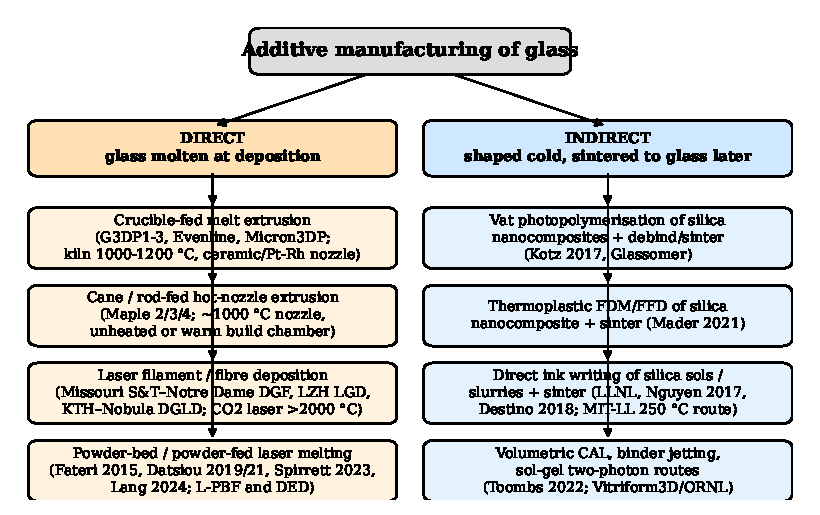
\includegraphics[width=\linewidth]{fig_taxonomy.pdf}
  \caption{Process taxonomy of glass additive manufacturing used in this review. The left branch (direct) groups processes in which the glass is in a liquid or viscous-liquid state when it is laid down or consolidated; the right branch (indirect) groups processes in which a silica-loaded polymer or sol is shaped at low temperature and converted to glass by debinding and sintering. The direct branch is the subject of this review. Representative systems and publications are named in each box; the sub-branches differ in feedstock (bulk melt, rod or cane, fibre, powder) and in heat source (resistive kiln, hot nozzle, CO$_2$ laser). Sources: \citet{klein2015,inamura2018,mit2024masonry,luo2017sodalime,witzendorff2018,kth2022bonding,fateri2015,datsiou2019,spirrett2023,lang2024,kotz2017,mader2021,nguyen2017,destino2018,toombs2022,ornl2026}.}
  \label{fig:taxonomy}
\end{figure}

Within the direct branch four sub-families are distinguished by feedstock and heat source:

\begin{enumerate}[leftmargin=*,itemsep=2pt]
  \item \textbf{Crucible-fed melt extrusion.} A charge of glass (\SIrange{2}{30}{kg}) is held molten in a refractory crucible inside an electric kiln at \SIrange{1000}{1200}{\celsius}; the melt drains under its own hydrostatic head through a heated ceramic (alumina or alumina--zirconia--silica) nozzle of \SIrange{5}{15}{mm} bore into a build chamber held near the annealing point. This is the G3DP lineage \citep{klein2015,inamura2018,mit2024masonry,patent_us10266442,patent_us9919510} and it is the only route that has produced architectural-scale parts (\SI{3}{m} columns, full-size masonry units). Deposition rates are \SIrange{2}{5}{kg/h}.
  \item \textbf{Cane- or rod-fed hot-nozzle extrusion.} A solid glass rod (``cane'') of a few millimetres diameter is pushed mechanically into a short heated nozzle at roughly \SI{1000}{\celsius} and extruded as a filament of \SIrange{0.5}{2}{mm}, analogous to polymer fused-filament fabrication. Only the last few millimetres of feedstock are molten at any time, so the thermal inertia and electrical power are small. This is the Micron3DP and Maple Glass Printing approach \citep{micron3dp_acers,maple_ammedia,threednatives2025}; the abandoned Corning application describes an induction-heated platinum--rhodium variant of the same idea \citep{patent_corning2021}.
  \item \textbf{Laser filament or fibre deposition.} A glass fibre (\SIrange{0.1}{0.2}{mm}) or rod (\SIrange{1}{3}{mm}) is fed into the focus of a CO$_2$ laser (\SI{10.6}{\micro\metre}, strongly absorbed by silicates) where it melts at \SIrange{1700}{2200}{\celsius} and wets the substrate or the previous layer. Because heating is non-contact there is no nozzle in contact with the melt and fused silica becomes printable. The process is called filament-fed or ``digital glass forming'' (DGF) by the Missouri S\&T--Notre Dame group \citep{luo2017sodalime,luo2018quartz,kinzel2025dgf}, laser glass deposition (LGD) by Laser Zentrum Hannover \citep{witzendorff2018,lgd2021coaxial,lgd2024homog}, and direct glass laser deposition (DGLD) by KTH and its spin-off Nobula \citep{kth2022bonding,kth2024microlens,nobula_web}.
  \item \textbf{Laser melting of powder (bed or blown).} Soda-lime, borosilicate or silica powder is melted track-by-track by a fibre or CO$_2$ laser either in a powder bed (L-PBF/SLM) \citep{fateri2015,khmyrov2016,datsiou2019,datsiou2021,slmirregular2023,boro2025laser} or blown coaxially into a melt pool (powder-fed directed energy deposition, DED) \citep{spirrett2023,lang2024}. The glass is molten locally, so the process belongs to the direct branch, but the short melt lifetime and the entrapped inter-particle gas leave porosity of the order of \SIrange{5}{12}{\percent} and opaque parts unless a very high energy input is used.
\end{enumerate}

A hybrid fifth category, \textbf{paste extrusion with in-situ laser melting}, deposits a water-based silica paste and immediately fuses it with a CO$_2$ laser, obtaining transparent fused silica without a furnace step \citep{ieee2019dlm,paste2024}. It is treated together with powder-fed DED.

\subsection{Why molten deposition is hard: the three couplings}
The difficulty of the direct route can be stated in one sentence: the same temperature field that must keep the glass fluid enough to flow and bond must also be steep enough to freeze the deposited cord before it slumps, and shallow enough at the end of the build to avoid thermal stress. Three couplings follow.

\emph{Rheology--geometry coupling.} The viscosity of a silicate melt changes by a decade for every \SIrange{40}{80}{\celsius} in the working range (\cref{sec:physics}). A nozzle-exit temperature of \SI{990}{\celsius} in G3DP corresponds to \(\eta \approx 640\,\)Pa\,s \citep{klein2015}; a \SI{350}{\celsius} drop across the five most recent layers, measured by infrared thermography, raises the viscosity by five orders of magnitude and is what stabilises the wall against its own weight \citep{klein2015}. Any drift in nozzle temperature therefore changes bead width, slump and layer bonding simultaneously.

\emph{Thermal--mechanical coupling.} Glass has no ductility. A temperature difference across a wall that exceeds roughly \SI{100}{\celsius} during cooling through the transformation range produces residual tensile stress that fractures the part on cooling or later in service. Molten deposition thus either requires a build chamber held near the annealing point (G3DP, \SIrange{480}{525}{\celsius}) or a heated build plate and post-anneal (laser processes, \SIrange{250}{600}{\celsius}) \citep{klein2015,inamura2018,luo2017sodalime,datsiou2019}.

\emph{Chemistry--hardware coupling.} Molten glass is a universal solvent for oxides. Every wetted component---crucible, nozzle, thermocouple sheath, build plate---is corroded, and the corrosion rate roughly doubles for each \SI{50}{\celsius} \citep{zircorr2025,pgm2010}. This is why crucible-fed machines are limited to soda-lime and (with difficulty) borosilicate glasses below \SI{1200}{\celsius}, why the Corning application specified an 80/20 platinum--rhodium nozzle \citep{patent_corning2021}, and why the fused-silica processes all use non-contact laser heating.

\subsection{Historical arc 2014--2026}
\Cref{fig:timeline} places the principal milestones on a common axis. The first period (2014--2018) was one of demonstration: automated melt extrusion at MIT (G3DP, 2015; G3DP2 with \SI{25}{kg} reservoir and four-axis bed, 2017--2018), CO$_2$-laser rod and fibre feeding at Missouri S\&T (2014--2018), quartz-fibre laser deposition at Hannover (2018), and the first commercial announcements by Micron3DP (Israel, 2015--2017). The second period (2019--2022) added the powder-bed and blown-powder variants in commercial L-PBF machines at Nottingham, systematic process-window studies of laser filament printing at KTH, and the emergence of desktop cane-fed machines from Maple Glass Printing (Melbourne, first machines 2022). The third period (2023--2026) is characterised by industrial translation and control: Evenline's third-generation G3DP3 with infrared monitoring and \SI{1200}{\celsius} capability printing recycled container and float glass and full-size interlocking masonry \citep{stern2024cgc,mit2024masonry}, Nobula's DGLD desktop printer reaching \SI{2200}{\celsius} \citep{nobula_aniwaa}, real-time thermal-camera closed-loop control of laser power in digital glass forming \citep{dgf2026control,lgd2025tempctrl}, and surface finishes of \SI{21}{nm} \(R_a\) on as-printed fused silica \citep{lgd2024homog}.

\begin{figure}[htbp]
  \centering
  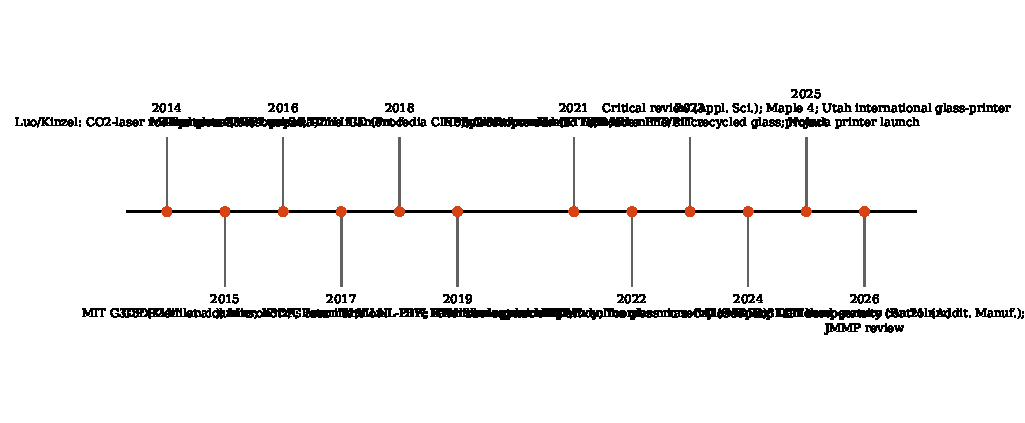
\includegraphics[width=\linewidth]{fig_timeline.pdf}
  \caption{Milestones of molten-glass additive manufacturing, 2014--2026, drawn from the harvested corpus. Events above the axis are academic, below the axis predominantly commercial or applied. Only first reports and first public machine releases are shown; incremental papers are cited in the relevant sections.}
  \label{fig:timeline}
\end{figure}

\subsection{Structure of the review}
\Cref{sec:physics} treats the materials physics: viscosity--temperature relations of the four glass families used, capillary and viscous-thread instabilities of the extruded cord, and transient heat transfer. \Cref{sec:hardware} reviews hardware: crucibles, nozzles and their materials, kiln architectures, laser heads, feed mechanisms and kinematics, and gives the modality comparison matrix (\cref{tab:modalities}). \Cref{sec:monitoring} covers in-situ thermal management, monitoring and annealing. \Cref{sec:open} formulates the open problems as explicit problem statements. \Cref{sec:academic,sec:industry} map the academic and industrial landscapes with the two directory tables, and \cref{sec:outlook} closes with a roadmap.

\section{Thermal regimes, materials and fluid dynamics}
\label{sec:physics}

\subsection{Viscosity--temperature behaviour of printable glasses}
The single most important material function in molten glass AM is the viscosity curve \(\eta(T)\). Over the whole range from the strain point (\(\eta = 10^{14.5}\,\)dPa\,s) to the melting range (\(\eta \sim 10^{2}\,\)dPa\,s) it is described to within a few kelvin by the Vogel--Fulcher--Tammann (VFT) equation \citep{fluegel2007,mauro2009},
\begin{equation}
  \log_{10}\eta = A + \frac{B}{T - T_0},
  \label{eq:vft}
\end{equation}
with \(\eta\) in dPa\,s (poise), \(T\) in kelvin, and three composition-dependent constants. \(A\) is the logarithm of the infinite-temperature viscosity, which for silicate melts is nearly universal at \(\log_{10}(\eta_\infty/\mathrm{Pa\,s}) \approx -2.9\) \citep{mauro2009}; \(B\) sets the fragility and \(T_0\) the divergence temperature, typically \SIrange{100}{300}{\celsius} below \(\Tg\). The glass industry defines four reference points on this curve, and every printing process can be located with respect to them:

\begin{itemize}[leftmargin=*,itemsep=1pt]
  \item strain point, \(\log_{10}\eta = 14.5\): below this, stress relaxation takes hours to days; the safe end of annealing;
  \item annealing point, \(\log_{10}\eta = 13.0\): stress relaxes in about 15 minutes; build chambers of crucible-fed printers are held \SIrange{20}{40}{\celsius} below it;
  \item Littleton softening point, \(\log_{10}\eta = 7.6\): a fibre deforms under its own weight; the upper bound for a deposited cord to retain shape;
  \item working point, \(\log_{10}\eta = 4.0\): the viscosity of hand-gathering and machine forming; nozzle-exit viscosities in melt extrusion are \(10^{3}\)--\(10^{4.5}\)\,dPa\,s, i.e.\ at or slightly above the working point.
\end{itemize}

\Cref{fig:vft} shows VFT fits for the four glass families relevant to the field, constructed from manufacturer fixed points \citep{valleydesign_sls,schott_borofloat,corning_eaglexg,heraeus_quartz}. For soda-lime float and BOROFLOAT~33 four points are available and all three constants were fitted; for the alkaline-earth boro-aluminosilicate (EAGLE XG) and fused silica only strain, annealing and softening points are published, so \(A\) was fixed at the universal value and \(B\), \(T_0\) fitted. The resulting constants are listed in \cref{tab:vft}. The fitted soda-lime constants (\(A=-2.39\), \(B=\SI{5210}{K}\), \(T_0=\SI{206}{\celsius}\)) agree well with the constants that Evenline derived for studio and recycled soda-lime glasses through the Fluegel composition model (\(A=-2.47\) to \(-2.67\), \(B=\SIrange{3965}{4488}{K}\), \(T_0=\SIrange{199}{278}{\celsius}\) with \(\eta\) in Pa\,s) \citep{stern2024cgc}; the different units shift \(A\) by one.

\begin{figure}[htbp]
  \centering
  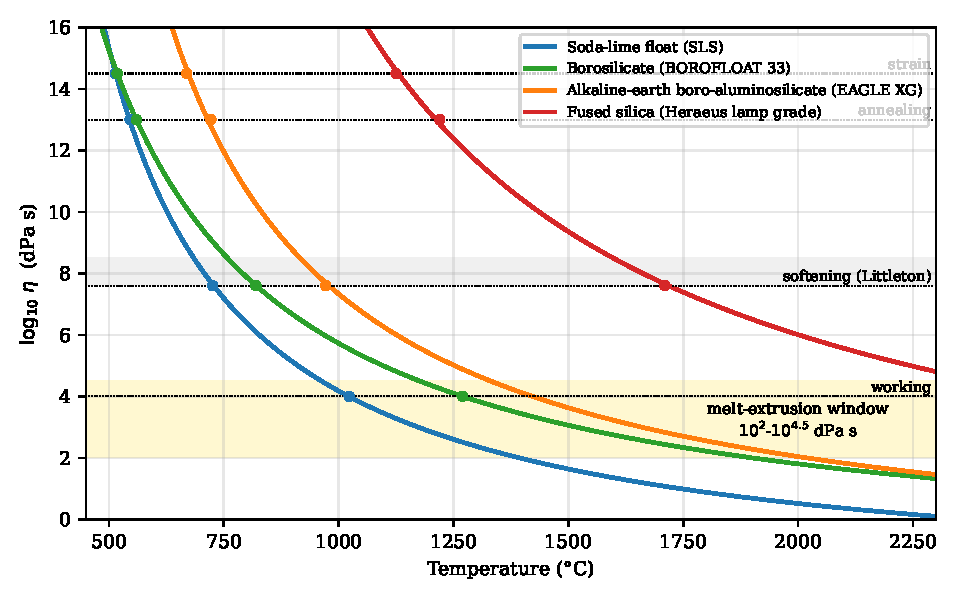
\includegraphics[width=\linewidth]{fig_vft_viscosity.pdf}
  \caption{Vogel--Fulcher--Tammann viscosity curves of the four glass families used in molten glass AM, fitted to published fixed points (markers): soda-lime float \citep{valleydesign_sls}, BOROFLOAT~33 \citep{schott_borofloat}, EAGLE XG \citep{corning_eaglexg} and lamp-grade fused silica \citep{heraeus_quartz}. Horizontal dotted lines mark the strain, annealing, softening and working points. The shaded band \(10^{2}\)--\(10^{4.5}\)\,dPa\,s is the viscosity window within which gravity-fed and cane-fed melt extrusion operates; it is reached at about \SI{1000}{\celsius} for soda-lime, \SI{1250}{\celsius} for borosilicate, \SIrange{1300}{1400}{\celsius} for boro-aluminosilicate and above \SI{2000}{\celsius} for fused silica, which is why the last is accessible only to laser heating. The fused-silica curve above the softening point is an extrapolation of the fixed-point fit and is consistent with the direct measurements compiled by Doremus \citep{doremus2002}.}
  \label{fig:vft}
\end{figure}

\begin{table}[htbp]
  \centering\small
  \caption{VFT constants (\(\eta\) in dPa\,s, \(T\) in K, \(T_0\) quoted in \si{\celsius}) fitted to manufacturer fixed points, and the temperatures at which each glass reaches the melt-extrusion viscosity \(10^{4}\)\,dPa\,s. Fits with \(A\) fixed at \(-1.93\) (universal \(\eta_\infty\) \citep{mauro2009}) are marked \(^{\dagger}\). Generated by \texttt{scripts/make\_figures.py}.}
  \label{tab:vft}
  \begin{tabular}{@{}lS[table-format=-1.2]S[table-format=5.0]S[table-format=-3.0]S[table-format=4.0]l@{}}
    \toprule
    Glass & {\(A\)} & {\(B\) (K)} & {\(T_0\) (\si{\celsius})} & {\(T(10^{4}\,\mathrm{dPa\,s})\) (\si{\celsius})} & Fixed-point source\\
    \midrule
    Soda-lime float & -2.39 & 5210 & 206 & 1023 & \citep{valleydesign_sls,stern2024cgc}\\
    BOROFLOAT~33 (borosilicate) & -1.68 & 6578 & 112 & 1270 & \citep{schott_borofloat}\\
    EAGLE XG (boro-aluminosilicate)\(^{\dagger}\) & -1.93 & 6947 & 250 & {1300--1420 (extrap.)} & \citep{corning_eaglexg}\\
    Fused silica (lamp grade)\(^{\dagger}\) & -1.93 & 13351 & 317 & {\(>\)2000 (extrap.)} & \citep{heraeus_quartz,doremus2002}\\
    \bottomrule
  \end{tabular}
\end{table}

Two practical consequences follow from \cref{fig:vft}. First, the \emph{working range}, defined by Evenline as the interval between working and softening points, is remarkably constant at \SI{295 +- 12}{\celsius} across six soda-lime compositions from studio batch to recycled float \citep{stern2024cgc}. This is why a single crucible-fed machine can be recalibrated for a new soda-lime source by ``viscosity matching'': setting the two VFT expressions equal and solving for the temperature of the new glass that gives the same viscosity as a proven set point,
\begin{equation}
  T_2 = T_{0,2} + \frac{B_2\,(T_1 - T_{0,1})}{B_1 + (T_1 - T_{0,1})(A_1 - A_2)},
  \label{eq:viscmatch}
\end{equation}
which predicted an Optifloat set point of \SI{1037}{\celsius} from a Spruce Pine PWV set point of \SI{1023}{\celsius} and produced a part mass within \SI{3.2}{\percent} of prediction at first attempt \citep{stern2024cgc}. Second, the slope \(\mathrm{d}\log_{10}\eta/\mathrm{d}T\) at the working point is about \SI{-0.012}{\per\kelvin} for soda-lime, so a \SI{10}{\celsius} error in nozzle temperature changes the gravity-fed flow rate by roughly \SI{30}{\percent} through \cref{eq:hp} below. Thermal control to \(\pm\)\SI{3}{\celsius} at the nozzle is therefore a hard requirement, not a refinement.

\subsection{Flow through the nozzle: Hagen--Poiseuille gravity feed}
In crucible-fed machines the melt is driven only by its own head. Klein et al.\ showed that with \(\eta \approx 640\,\)Pa\,s, \(\rho \approx \SI{2400}{\kilogram\per\cubic\metre}\), \(d = \SI{10}{mm}\) and \(v \approx \SI{6}{mm/s}\) the Reynolds number is \(Re = \rho v d/\eta \approx 2\times10^{-4}\), so the flow is creeping (Stokes) flow and the Hagen--Poiseuille law applies segment by segment \citep{klein2015,inamura2018}:
\begin{equation}
  Q = \frac{\Delta P}{R}, \qquad R = \sum_i \frac{8\,\eta\, L_i}{\pi r_i^{4}}, \qquad \Delta P = \rho g H .
  \label{eq:hp}
\end{equation}
Because \(R \propto r^{-4}\), more than half of the total resistance of the G3DP crucible--nozzle assembly resided in the final \SI{10}{mm} bore, and a head of \(H = \SI{80}{mm}\) (\(\Delta P \approx \SI{3.6}{kPa}\)) gave a linear exit velocity of \SI{5.7}{mm/s} \citep{klein2015}. G3DP2 lengthened the nozzle for insulation but widened it to obtain a net \SI{17}{\percent} lower resistance and doubled the head, more than doubling the flow to \SI{5.2}{kg/h} (\SI{570}{mm^3/s}) \citep{inamura2018}. The linear dependence of \(Q\) on \(H\) is also the principal source of drift in gravity-fed printing: as the crucible empties, the bead narrows, which is why G3DP required refilling every few minutes and why G3DP2 raised the reservoir-to-print-volume ratio from \SI{4.6}{\percent} to \SI{29}{\percent} \citep{inamura2018}. Cane-fed and filament-fed machines avoid this problem entirely because the volumetric feed rate is set by the feeder motor, \(Q = \pi r_{\mathrm{cane}}^{2} v_{\mathrm{feed}}\), and the extruded bead cross-section then follows from mass conservation, \(A_{\mathrm{bead}} = Q / v_{\mathrm{travel}}\); over-feeding by \SI{50}{\percent} relative to the geometric requirement was found necessary in laser filament printing to obtain good wetting of the previous layer \citep{kth2022bonding}.

\subsection{Capillary instabilities of the molten cord}
A cylinder of liquid of radius \(a\) and surface tension \(\sigma\) is unstable to axisymmetric perturbations of wavelength \(\lambda > 2\pi a\) (Plateau's criterion). Rayleigh's inviscid analysis \citep{rayleigh1878} gives the growth rate \(\omega\) of a perturbation of wavenumber \(k\) as
\begin{equation}
  \omega^{2} = \frac{\sigma}{\rho a^{3}}\, \frac{x\, I_1(x)}{I_0(x)}\,(1 - x^{2}), \qquad x = ka,
  \label{eq:rayleigh}
\end{equation}
with \(I_n\) the modified Bessel functions. The fastest-growing mode is at \(x \simeq 0.697\), i.e.
\begin{equation}
  \lambda_{\mathrm{opt}} \simeq 9.02\,a \simeq 4.51\, d_{\mathrm{filament}},
  \label{eq:lambdaopt}
\end{equation}
the classical result that a jet breaks into drops spaced by about four and a half diameters \citep{rayleigh1878,tomotika1935,wiki_plateau}. For molten glass, however, the relevant limit is the opposite one. The Ohnesorge number \(Oh = \eta/\sqrt{\rho\sigma a}\) for a \SI{10}{mm} soda-lime cord at \SI{1000}{\celsius} (\(\eta \approx 10^{3}\,\)Pa\,s, \(\sigma \approx \SI{0.32}{\newton\per\metre}\), \(\rho = \SI{2400}{\kilogram\per\cubic\metre}\)) is of order \(10^{3}\), and for a \SI{200}{\micro\metre} fused-silica fibre at \SI{2000}{\celsius} (\(\eta \approx 10^{4.5}\,\)Pa\,s) it is of order \(10^{6}\). Inertia is irrelevant and the Stokes-limit dispersion relation for a viscous thread \citep{tomotika1935} applies,
\begin{equation}
  \omega = \frac{\sigma}{2\eta a}\;\frac{1 - x^{2}}{x^{2}\,[I_0(x)/I_1(x)]^{2} - x^{2} - 1},
  \qquad \omega(x\to 0) \to \frac{\sigma}{6\,\eta\, a},
  \label{eq:tomotika}
\end{equation}
which has no interior maximum: the growth rate increases monotonically toward long wavelengths and its magnitude is set by the visco-capillary time \(\tau_{vc} = \eta a/\sigma\). \Cref{fig:rp} contrasts the two limits. For the G3DP cord \(\tau_{vc} \approx 10^{3}\times 5\times10^{-3}/0.32 \approx \SI{16}{s}\) at the nozzle exit, growing to \(10^{5}\)\,s within a few layers as the glass cools by \SI{350}{\celsius}; capillary break-up therefore never occurs, but the same visco-capillary time governs the \emph{healing} of the layer seam by surface tension. For the laser-heated fibre \(\tau_{vc} \approx 3\times10^{4}\times10^{-4}/0.3 \approx \SI{10}{s}\), and the process must indeed avoid dwell times of this order at full temperature or the free length of fibre between feeder and melt pool necks and separates---the ``premature filament detachment'' failure mode reported for digital glass forming \citep{dgf2026control}.

\begin{figure}[htbp]
  \centering
  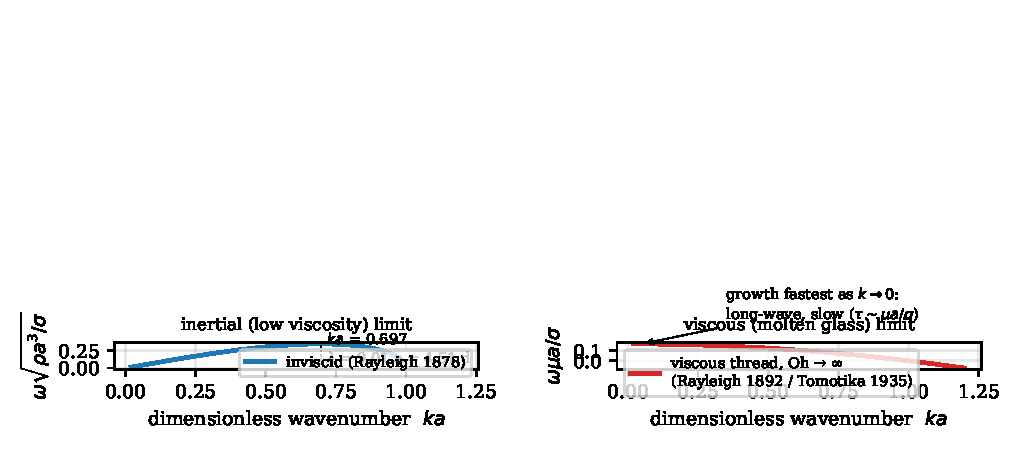
\includegraphics[width=\linewidth]{fig_rayleigh_plateau.pdf}
  \caption{Dispersion relations for the capillary instability of a liquid cylinder. Left: inviscid Rayleigh limit, \cref{eq:rayleigh}, with the most unstable wavelength \(\lambda_{\mathrm{opt}} = 4.51\,d\) marked. Right: Stokes (viscous-thread) limit, \cref{eq:tomotika}, relevant to molten glass cords for which \(Oh \gg 1\): the growth rate scales as \(\sigma/(\eta a)\) and is largest for the longest wavelengths, so break-up is slow and the deposited cord is preserved, but the same time scale controls seam healing. Sources: \citet{rayleigh1878,tomotika1935}.}
  \label{fig:rp}
\end{figure}

\subsection{Gravitational slump and the viscous-thread (coiling) instability}
Slumping of a freshly deposited cord under gravity is a competition between the gravitational stress \(\rho g h\) over a wall of height \(h\) and the viscous resistance; the characteristic sag velocity is \(v_{\mathrm{sag}} \sim \rho g h a^{2}/\eta\). With \(h = \SI{5}{mm}\), \(a = \SI{5}{mm}\) and \(\eta = 10^{3}\,\)Pa\,s this is \SI{3}{mm/s} at the nozzle exit and falls to \SI{3}{\micro\metre/s} once the viscosity has risen five decades: the wall is self-supporting only because the cooling is fast relative to the layer time. This is the origin of the empirical overhang limit of \SIrange{30}{35}{\degree} and the minimum turning radius of \SIrange{6}{15}{mm} of the G3DP machines \citep{klein2015,mit2024masonry}, and of the maximum layer height of \SI{5}{mm} at a \SI{10}{mm/s} feed rate.

When the nozzle is lifted well above the bed, the falling cord buckles and coils, the ``fluid-mechanical sewing machine''. Brun et al.\ rationalised the patterns (meanders, alternating loops, translated coiling) in terms of the dimensionless fall height \(H = H^{*}(g/\nu^{2})^{1/3}\) and belt speed \(V = V^{*}/(g\nu)^{1/3}\), with \(\nu\) the kinematic viscosity, and used a geometrical model to program the coiling of molten soda-lime glass at \SI{1070}{\celsius} into uniformly sized building blocks \citep{brun2017,klein2015}. A G3DP cylinder printed at \(H^{*} = \SI{100}{mm}\) (\(H = 1.02\), \(V = 0.003\)) reproduced translated coiling with loops of consistent radius and pitch, verified by micro-computed tomography \citep{klein2015}. The same instability is now exploited on polymer printers to make graded foams \citep{vti2022}; in glass it offers a route to multiscale lattices whose optical scattering is set by the coil pitch rather than by the layer height.

\subsection{Surface tension, Marangoni flow and wetting}
Surface tension of soda-lime melts is \SIrange{0.31}{0.33}{\newton\per\metre} between \SI{1200}{\celsius} and \SI{1400}{\celsius}, and its temperature coefficient is small and, unusually, positive for many complex silicate liquids \citep{fluegel2007}. In crucible-fed extrusion the temperature gradients across the cord are modest and Marangoni stresses are negligible compared with viscous stresses; the dominant interfacial effect is instead \emph{wetting of the nozzle face}. Molten glass adheres to the alumina nozzle tip, and when the adhering film is asymmetric it exerts an off-axis pull on the just-deposited cord, distorting the wall at convexity changes; G3DP2 reduced this by raising the nozzle tip cone angle from \SIrange{30}{45}{\degree} to reduce the contact area \citep{inamura2018}. In laser melt pools the situation is reversed: intensity gradients of the focused beam produce surface-temperature gradients of \(10^{3}\)--\(10^{4}\)\,K/mm, and Marangoni convection and evaporation recoil determine the melt-pool shape and the surface topography of laser-formed optical glass \citep{machines2026meltpool}. Excess laser power in fibre printing produces visible fumed-silica deposits from vapour condensation, whereas insufficient power leaves ``wiggly'' lines because the fibre does not wet the substrate \citep{kth2022bonding}. Bonding width (the wetted contact width between a \SI{196}{\micro\metre} fibre and a fused-quartz substrate) rises with laser power from \SI{17}{\micro\metre} and saturates near \SI{221}{\micro\metre}, while layer-to-layer bonding widths of \SI{99 +- 12}{\micro\metre} were obtained in 105-layer walls \citep{kth2022bonding}.

\subsection{Transient heat transfer and cooling of the deposited cord}
A deposited cord loses heat by radiation and convection to the chamber and by conduction into the layer below. For a cord of diameter \(d\) whose Biot number is small (\(Bi = h_{\mathrm{eff}} d / 2k \lesssim 0.3\), which holds for \(d \lesssim \SI{15}{mm}\) with \(k \approx \SI{1.4}{\watt\per\metre\per\kelvin}\) and radiative \(h_{\mathrm{eff}} \approx \SIrange{50}{100}{\watt\per\square\metre\per\kelvin}\) at \SI{1000}{\celsius}), a lumped energy balance gives
\begin{equation}
  \rho c_p \frac{d}{4}\,\frac{\mathrm{d}T}{\mathrm{d}t} = -\,h\,(T - T_\infty) - \varepsilon\sigma_{\mathrm{SB}}\,(T^{4} - T_\infty^{4}),
  \label{eq:cooling}
\end{equation}
with emissivity \(\varepsilon \approx 0.9\) for glass in the thermal infrared. \Cref{fig:cooling} integrates \cref{eq:cooling} for soda-lime cords of \SIrange{2}{15}{mm} released at \SI{1050}{\celsius} into a chamber at \SI{520}{\celsius} (crucible-fed architecture) and into ambient air (cane-fed desktop architecture). Two regimes emerge. In the heated chamber a \SI{10}{mm} cord falls below the softening point in about \SI{25}{s} and then asymptotes to the chamber temperature, never entering the stress-generating region below the annealing point until the programmed anneal; this reproduces the measured \SI{350}{\celsius} drop across five layers at a \SI{4.5}{mm}, \SI{6}{mm/s} layer schedule (about \SI{50}{s} per layer for a \SI{300}{mm} perimeter) \citep{klein2015}. In open air a \SI{2}{mm} cane-fed filament crosses the softening point in \SI{2}{s} and the annealing point in \SI{4}{s}; the part is therefore built as an already rigid, stressed body, which is why cane-fed desktop machines rely on rapid solidification for overhangs and bridges \citep{maple_ammedia} but must anneal afterwards, and why their wall thicknesses are limited to a few millimetres. For 1-D conduction into a semi-infinite substrate the interface temperature after contact is the contact temperature \(T_c = (T_1 e_1 + T_2 e_2)/(e_1 + e_2)\) with effusivities \(e = \sqrt{k\rho c_p}\); for glass on glass this is simply the mean of cord and previous-layer temperatures, so a \SI{990}{\celsius} cord landing on a \SI{700}{\celsius} layer produces an \SI{845}{\celsius} interface (\(\eta \approx 10^{5}\)\,dPa\,s)---fluid enough to fuse, which is consistent with the SEM observation of a blunt, featureless interlayer interface in annealed G3DP samples \citep{klein2015}.

\begin{figure}[htbp]
  \centering
  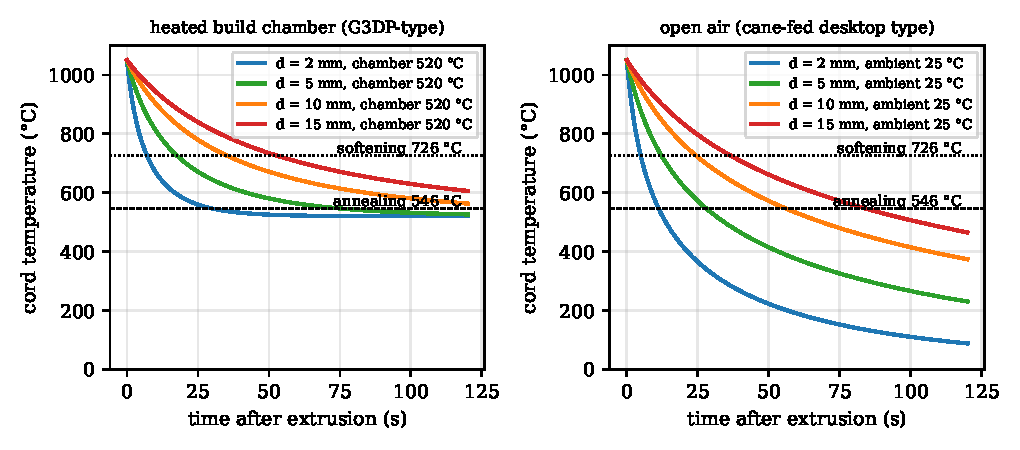
\includegraphics[width=\linewidth]{fig_cord_cooling.pdf}
  \caption{Lumped radiative--convective cooling, \cref{eq:cooling}, of soda-lime cords of \SI{2}{}--\SI{15}{mm} diameter released at \SI{1050}{\celsius} (\(\rho=\SI{2500}{\kilogram\per\cubic\metre}\), \(c_p=\SI{1200}{\joule\per\kilogram\per\kelvin}\), \(\varepsilon=0.9\), \(h=\SI{15}{\watt\per\square\metre\per\kelvin}\)). Left: into a build chamber at \SI{520}{\celsius}, as in the G3DP family; the cord stays above the annealing point. Right: into ambient air, as in cane-fed desktop printers; thin filaments pass through the transformation range within seconds and accumulate residual stress that must be removed by a post-anneal. The softening (\SI{726}{\celsius}) and annealing (\SI{546}{\celsius}) points of float glass are marked.}
  \label{fig:cooling}
\end{figure}

In laser filament processes the energy balance is local. Luo et al.\ estimated melt-pool temperature from a low-order balance between absorbed laser power, radiative loss and conduction along the filament and into the substrate, validated against incandescence spectra; the model predicts the onset of ``reboil'' (bubble nucleation from dissolved gases and sulfate decomposition) above a threshold temperature and the incomplete fusion (index inhomogeneity) below it \citep{luo2017heat,luo2017sodalime}. For fused silica the window is bounded below by roughly \SI{1900}{\celsius} for wetting and above by evaporation, which becomes measurable near \SI{2200}{\celsius} \citep{witzendorff2018,kth2022bonding}. Because the thermal conductivity of glass is low, heat delivered to the top of a thick filament diffuses slowly to the interface; injecting the laser from the side so that it heats the filament--substrate junction directly was shown to raise the achievable deposition rate \citep{capps2021interface}.

\subsection{Thermal stress and the annealing requirement}
When a glass wall cools through the transformation range with a through-thickness temperature difference \(\Delta T\), the frozen-in stress is of order
\begin{equation}
  \sigma_{\mathrm{res}} \approx \frac{E\,\alpha\,\Delta T}{2(1-\nu_{\mathrm{P}})},
  \label{eq:stress}
\end{equation}
which for soda-lime (\(E = \SI{70}{GPa}\), \(\alpha = \SI{9e-6}{\per\kelvin}\), \(\nu_{\mathrm{P}} = 0.22\)) is \SI{40}{MPa} per \SI{100}{\celsius}---comparable to the practical tensile strength of glass (\SIrange{40}{80}{MPa}) \citep{inamura2018}. This is why samples printed at room temperature in the first G3DP experiments showed radial residual stress under the polariscope and a flexural strength one fifth of that of samples printed into the heated chamber \citep{klein2015}, and why fused silica, with \(\alpha = \SI{0.5e-6}{\per\kelvin}\), tolerates the extreme gradients of laser deposition that would shatter soda-lime or borosilicate \citep{luo2018quartz,lgd2021coaxial}. The annealing schedule is set by the relaxation time \(\tau = \eta/G\) (\(G \approx \SI{30}{GPa}\)): \SI{15}{min} at the annealing point, hours at the strain point, and a cooling rate below it that keeps \(\Delta T\) small; Evenline's masonry units of \SI{13}{mm} wall thickness were annealed with schedules of several hours, and the fully printed variants with thicker bases required longer cycles \citep{mit2024masonry}.

\section{Hardware: crucibles, nozzles, laser heads and kinematics}
\label{sec:hardware}

\subsection{Crucible-fed melt extrusion: the G3DP architecture}
\Cref{fig:g3dp} shows the generic architecture of a crucible-fed molten glass printer as embodied by G3DP (2015), G3DP2 (2017--2018) and G3DP3 (2023--present). Three independently controlled thermal zones are stacked vertically and decoupled mechanically from the motion system.

\begin{figure}[htbp]
  \centering
  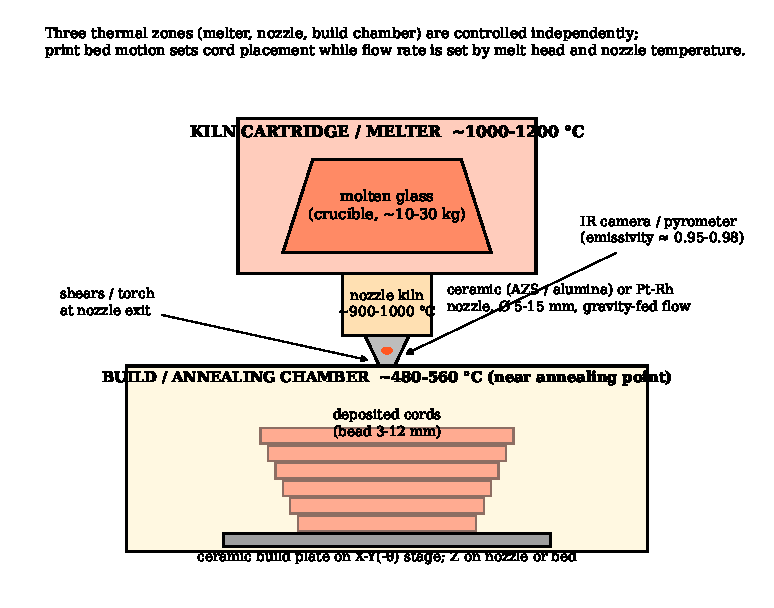
\includegraphics[width=0.9\linewidth]{fig_g3dp_schematic.pdf}
  \caption{Schematic of a crucible-fed molten-glass extrusion printer of the G3DP type. A refractory crucible in an electric kiln (melter, \SIrange{1040}{1200}{\celsius}) drains under its own head through a separately heated ceramic nozzle (\SIrange{800}{1010}{\celsius}) into an electrically heated build chamber held near the annealing point (\SIrange{480}{525}{\celsius}); the build plate moves in X--Y(--\(\theta\)) and Z. Flow is initiated and terminated by a concentric gas torch and compressed-air ring at the nozzle tip; an infrared camera views the cord through a ceramic-glass window. Dimensions and temperatures from \citet{klein2015,inamura2018,mit2024masonry,patent_us9919510}.}
  \label{fig:g3dp}
\end{figure}

\paragraph{Melter.} G3DP used an \SI{1800}{W} alumina--silica fibreboard kiln with FeCrAl wire heating a refractory crucible of \SI{2.1}{kg} capacity at \SIrange{1040}{1165}{\celsius}; the charge was either melted from nuggets over four hours and fined for two hours, or ladled in molten from a furnace \citep{klein2015}. G3DP2 replaced this with a \SI{6.5}{kW} kiln and a custom cast-alumina crucible of \SI{25.5}{kg} capacity operating at \SI{1090}{\celsius}, raising the reservoir-to-print-volume ratio from \SI{4.6}{\percent} to \SI{29}{\percent} and eliminating in-print refilling \citep{inamura2018}. The MIT patent describes idle and print set points of \SI{1750}{\degree}F and \SI{1850}{\degree}F (\SI{954}{\celsius} and \SI{1010}{\celsius}) for the melter, with silicon-carbide resistive heaters and type-S thermocouples \citep{patent_us9919510}. G3DP3 raised the maximum extrusion temperature to \SI{1200}{\celsius} and lowered the cost of the crucible and refractories \citep{mit2024masonry}; the feedstock kiln for recycled container glass is a separate double-walled crucible kiln conditioned at \SIrange{1190}{1218}{\celsius} for twelve hours before gathering \citep{stern2024cgc}.

\paragraph{Nozzle.} The nozzle is the interface between the thermal and kinematic systems and the component that limits campaign length. G3DP machined its nozzle from bulk alumina bisque, sealed to the crucible with refractory mortar, and heated it with a \SI{300}{W} nozzle kiln to \SI{1010}{\celsius} (\SI{800}{\celsius} to hold flow) \citep{klein2015}. G3DP2 used a solid-alumina nozzle of \SI{11.5}{mm} bore, lengthened for insulation and widened to keep resistance down, heated by resistive wire on a silicon-carbide mandrel in a structural refractory housing at \SI{800}{\celsius} idle and \SI{915}{\celsius} to start flow; a concentric gas manifold at the tip either burns propane to initiate flow or blows compressed air to freeze it, and the tip cone angle was increased from \SIrange{30}{45}{\degree} to reduce asymmetric wetting \citep{inamura2018}. Even so, nozzle joinery dictated print campaigns of two to three weeks \citep{inamura2018}. The press coverage of G3DP describes the nozzle material as alumina--zirconia--silica (AZS) \citep{oxman_platform}, the fused-cast refractory whose corrosion mechanism (alkali diffusion into the glassy phase, exudation, pore formation) has been reviewed recently \citep{zircorr2025}. G3DP3 redesigned the nozzle for higher temperature and for a \SI{13}{mm} nominal wall \citep{mit2024masonry,stern2024cgc}. Evenline's public machine description is a ceramic nozzle printing at \SI{2000}{\degree}F (\SI{1093}{\celsius}) \citep{evenline_web}.

\paragraph{Build chamber.} G3DP printed into a \SI{3300}{W} kiln derived from a Skutt GlazeTech, with a Neoceram ceramic-glass window and fibreboard skirts sealing the moving carriage \citep{klein2015}. G3DP2's chamber is a \SI{12}{kW} kiln of \qtyproduct{1100 x 1100 x 500}{mm} interior held at \SI{480}{\celsius}, with double-pane Neoceram doors and a \qtyproduct{400 x 400}{mm} floor opening through which the print-bed support tube passes; a \SI{13}{mm} Duraboard shield on the Z-actuator seals the opening while the bed translates and rotates \citep{inamura2018}. Total power of the G3DP2 thermal module is \SI{19}{kW} peak and \SI{15}{kW} during printing \citep{inamura2018}. After printing the object is soaked at \SI{525}{\celsius} for about five minutes and transferred to an external annealing oven so that the printer can be reused \citep{inamura2018}.

\paragraph{Kinematics.} G3DP moved the entire kiln cartridge on a steel carriage in X--Y with stepper motors (\SI{280}{\newton\centi\metre} holding torque) and moved the bed in Z, controlled by an Arduino/RAMPS stack and Repetier firmware \citep{klein2015}. G3DP2 inverted the architecture: the thermal module is stationary and the bed moves on a four-axis CNC (THK KR-46 linear actuators, a Bell-Everman rotary stage, Teknic ClearPath closed-loop servos, TinyG controller) designed to a positional tolerance of \(\pm\)\SI{1.0}{mm}, i.e.\ \SI{10}{\percent} of the \SI{10}{mm} filament \citep{inamura2018}. The rotary A-axis keeps the deposition direction constant relative to the stationary nozzle so that the viscous cord is not sheared by a change of pull direction---the core claim of the MIT patents \citep{patent_us9919510,patent_us10464305}. Measured repeatability across ten \SI{200}{mm} cylinders was a diameter range of \SI{0.7}{mm} (\SI{0.3}{\percent}) with a mean shrinkage of \SI{1.4}{\percent} \citep{inamura2018}. Jerk-limited acceleration on the rotary axis caused wall thickening at inflection points, so production parts were printed with three axes \citep{inamura2018}. G3DP3's proven envelope is \qtyproduct{325 x 325 x 380}{mm}, bead height \SIrange{3.0}{6.0}{mm}, bead width \SIrange{9}{16}{mm}, feed rate \SIrange{6}{20}{mm/s}, minimum path radius \SIrange{6}{15}{mm}, maximum overhang \SIrange{30}{35}{\degree} \citep{mit2024masonry}.

\subsection{Cane-fed hot-nozzle extrusion}
The cane-fed architecture inverts the thermal-mass problem: instead of holding tens of kilograms molten, it melts only the tip of a solid rod. Maple Glass Printing's Maple~2 and Maple~3 (2022--2023) feed one-metre soda-lime canes mechanically into a stationary nozzle at \SIrange{900}{1000}{\celsius} and deposit onto a moving build plate; the \SI{1.5}{mm} nozzle lays down beads up to \SI{2.0}{mm} high with layer resolution down to \SI{0.1}{mm}, in a \qtyproduct{170 x 200 x 300}{mm} volume, and the whole machine draws less power than a hair dryer because only a few millimetres of glass are hot at any moment \citep{maple_ammedia,maple_aniwaa,threednatives2025}. The Maple~4 (2025) is a \qtyproduct{736 x 600 x 985}{mm}, \SI{100}{kg} desktop unit with a \qtyproduct{200 x 200 x 300}{mm} volume, mesh bed levelling, a magnetic bed and a nozzle approaching \SI{1000}{\celsius} \citep{threednatives2025,maple_web}. The company also built a ``Vitri-Glass'' cane-drawing machine that melts recycled cullet in a crucible and pulls cane to specification, closing the material loop, with the caveat that coloured cullet must be segregated \citep{maple_ammedia}. Micron3DP's earlier machines (2015--2021) used an all-metal high-temperature extruder with \SI{100}{\micro\metre} layers, a \qtyproduct{200 x 200 x 300}{mm} volume, and claimed soda-lime at \SI{850}{\celsius} and borosilicate at \SI{1640}{\celsius} \citep{micron3dp_acers,micron3dp_3dprint2017}; the technical details were withheld pending patents and the company's alpha units of 2017--2021 were not followed by a public product. Corning's 2016 application describes the industrial form of the concept: a barrel-and-nozzle crucible of 80/20 platinum--rhodium heated by induction, fed with rigid rods of \SI{1}{mm} to over \SI{125}{mm} diameter, extruding controlled beads onto a platform; it was abandoned without grant \citep{patent_corning2021}. Because the cord in a cane-fed machine is thin (\SIrange{0.5}{2}{mm}) it freezes within seconds in air (\cref{fig:cooling}); this permits bridges and overhangs but produces stressed parts that require a post-anneal, and it limits optical clarity because the many fine layer seams scatter light---an effect already noted in comparing the Micron3DP and G3DP outputs \citep{inamura2018}.

\subsection{Laser filament, fibre and rod deposition heads}
\Cref{fig:laserhead} shows the generic laser filament head. The CO$_2$ laser at \SI{10.6}{\micro\metre} is absorbed within a few micrometres of the glass surface, so the melt zone is heated from the outside and the process is limited by conduction through the low-conductivity filament.

\begin{figure}[htbp]
  \centering
  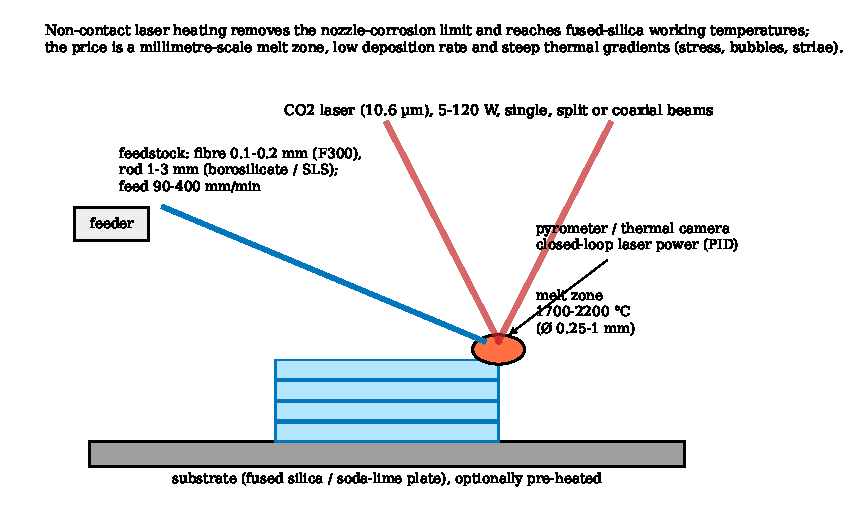
\includegraphics[width=0.85\linewidth]{fig_laser_filament_schematic.pdf}
  \caption{Schematic of a laser filament-fed glass deposition head (digital glass forming, laser glass deposition, direct glass laser deposition). A fibre or rod is fed at \SIrange{90}{400}{mm/min} into the focus of one or more CO$_2$ beams (\SIrange{5}{120}{W}); the melt zone of \SIrange{0.25}{1}{mm} diameter at \SIrange{1700}{2200}{\celsius} wets the substrate or previous layer. Melt-pool temperature is measured by pyrometry or thermal imaging and fed back to laser power. Parameters from \citet{luo2017sodalime,witzendorff2018,kth2022bonding,lgd2024homog,lgd2025tempctrl,dgf2026control}.}
  \label{fig:laserhead}
\end{figure}

\paragraph{Missouri S\&T / Notre Dame (digital glass forming).} The original 2014 system fed \SI{1}{mm} rods by hand into a CO$_2$ beam; automated feeding followed with soda-lime filaments \citep{luo2014jmse,luo2017sodalime}, then fused quartz filaments with spectroscopic and pyrometric measurement of the melt \citep{luo2018quartz,luo2016spie}, and stripped SMF-28 telecommunication fibre of \SI{125}{\micro\metre} as a kilometre-long, inexpensive, bubble-free feedstock \citep{hostetler2018fiber,hostetler2018sff}. The workpiece sits on a heated build platform on a four-axis stage; laser power, feed rate and scan speed are the three governing parameters, and the temperature window between incomplete fusion (index inhomogeneity) and reboil (bubbles) is narrow \citep{luo2017sodalime}. Side injection of the beam at the filament--substrate interface raised deposition rate \citep{capps2021interface}, hollow tubes were printed \citep{dgf2023tubes}, and the 2026 controller work replaced the pyrometer with a thermal camera on an RT-Linux platform and demonstrated that constant laser power fails on multilayer walls whereas closed-loop power succeeds \citep{dgf2026control}. The Notre Dame group also uses CO lasers and couples the process with ultrafast-laser machining in a hybrid cell \citep{notredame_dgf,kinzel2025dgf}.

\paragraph{Laser Zentrum Hannover (laser glass deposition).} The LGD process melts quartz-glass fibre with a combined laser head; at \SI{120}{W} a continuous regime was found up to feed and axis speeds of \SI{300}{mm/min}, above which the fibre outran the melt, and crack-free cylinders were built \citep{witzendorff2018}. A coaxial head with the fibre fed through the centre of a ring-shaped beam was introduced to make the process direction-independent and to reduce residual stress, supported by a thermal simulation of the fibre \citep{lgd2021coaxial}. A 3-axis linear system with integrated rotary axis, lateral fibre feed at a defined angle, an on-axis camera and a beam camera for transmitted-wavefront inspection form the current platform; fully dense fused-silica specimens without pores or boundary layers and with \(R_a = \SI{21}{nm}\) at \SI{90}{mm/min} feed (\SI{20}{}--\SI{40}{nm} up to \SI{126}{mm/min}; \SI{220}{nm} and waviness at \SI{180}{mm/min}; unmeasurable waviness at \SI{396}{mm/min}) were produced, with a contour flank angle of \SI{14}{\degree} as the price of the smoothest surface \citep{lgd2024homog,lgd2022fibers,grotesk2022}.

\paragraph{KTH / Nobula (direct glass laser deposition).} The KTH system uses four focused beams from a \SI{25}{W} CO$_2$ laser (\SIrange{2.2}{5.3}{W} delivered, stable to \SI{+-2}{\percent}) in a coaxial arrangement giving a \SIrange{250}{400}{\micro\metre} hot zone; \SI{196 +- 2}{\micro\metre} Heraeus F300 fibre drawn on a fibre tower is fed at \SI{150}{\percent} of the geometric rate at print speeds of \SIrange{10}{100}{mm/min} with \SI{200}{\micro\metre} layers onto a \qtyproduct{25 x 25}{mm} fused-quartz plate; a \qtyproduct{10.5 x 3.5 x 21}{mm}, 105-layer wall showed no stress birefringence and a material loss of \SI{-1.6 +- 2}{\percent} \citep{kth2022bonding}. The same head printed 5\(\times\)5 fused-silica microlens arrays in under ten seconds per lens with \(R_a = \SI{0.12}{nm}\) and uniform focal lengths \citep{kth2024microlens}. Nobula's commercial printer is specified at up to \SI{2200}{\celsius}, \qtyproduct{180 x 180 x 100}{mm}, \SI{0.1}{mm} Z resolution, \SIrange{100}{250}{\micro\metre} feature resolution and a \qtyproduct{1000 x 400 x 600}{mm}, \SI{50}{kg} footprint \citep{nobula_aniwaa,nobula_fabbaloo,threednatives2025}.

\paragraph{TU Ilmenau and TU Darmstadt (rod-fed).} Fr{\"o}hlich, Hildebrand and Bergmann used a CO$_2$ laser to create a melt pool on the substrate and fed borosilicate and soda-lime rods into it to build 3D structures \citep{froehlich2022}, and Seel et al.\ (TU Darmstadt) demonstrated ``fused glass deposition modelling'' of soda-lime rod onto float-glass plates for all-glass building connections \citep{seel2018}; a 2024 study designed printed glass point fixings on this basis \citep{pointfixings2024}. Both are relevant to the printing-on-sheet application that Evenline later demonstrated with a crucible-fed machine \citep{stern2024cgc}.

\paragraph{Coaxial wire and powder DED (IOE-CAS Chengdu, SCUT).} The Chinese Academy of Sciences group built a coaxial powder-fed laser DED head for quartz glass and reached \SI{72.4 +- 6.0}{MPa} flexural strength, \SI{95}{\percent} of conventional quartz \citep{lang2024}, then added coaxial wire feeding with PID closed-loop control of laser power from melt-pool temperature, which produced denser surfaces than constant powers of \SI{120}{W} or \SI{140}{W} \citep{lgd2025tempctrl}. The Clemson/SCUT route prints a water-based silica paste and melts it in situ with a CO$_2$ laser, avoiding a furnace step \citep{ieee2019dlm,paste2024}.

\subsection{Powder-bed and blown-powder laser melting hardware}
Nottingham's Centre for Additive Manufacturing processed soda-lime powder (\(\Tg = \SI{575}{\celsius}\), liquidus \SI{1280}{\celsius}) in a commercial fibre-laser L-PBF system with the substrate held at \SI{250}{\celsius} to limit thermal cracking; the process window was defined in terms of volumetric energy density \(E = P/(v\,h\,t)\), parts had \SI{12.1}{\percent} average porosity and a \SI{6.5}{MPa} mean flexural strength, and a \SI{650}{\celsius}, five-hour heat treatment improved translucency \citep{datsiou2019,datsiou2021}. Irregular (milled) soda-lime powder reached \SI{95}{\percent} relative density at Fudan \citep{slmirregular2023}; alkali-borosilicate powder was processed by Zeiss and TU Ilmenau over the whole window from open-pored (\SI{38}{\percent}) to vitrified (\SI{94}{\percent}) density, with characteristic ``vitrification strands'' from the line-wise energy input \citep{boro2025laser}; and Fateri and Gebhardt's 2014--2015 work reached \SI{93}{\percent} \citep{fateri2015}. Crack-free single beads and monolayers of silica glass on a silica substrate were shown by Khmyrov et al.\ \citep{khmyrov2016}. Blown-powder DED of soda-lime onto soda-lime bottles, with an adhesive tape layer to hold the powder on the transparent substrate and a cracking threshold at \SI{115}{W}, is proposed for one-step packaging decoration \citep{spirrett2023}. A finite-difference densification model predicts monolayer consolidation within \SI{2}{\percent} of experiment and shows that finer powder and higher preheat both help \citep{slmsim2024}.

\subsection{Comparison matrix of glass AM modalities}
\Cref{tab:modalities} summarises the quantitative envelope of each modality as reported in the corpus. The columns follow the specification of this review: temperature, build volume, deposition rate, optical clarity, surface roughness and strength.

\begin{sidewaystable}[p]
  \centering\scriptsize
  \caption{Comparison matrix of glass AM modalities. Direct (molten at deposition) modalities are listed first; indirect routes are included for contrast. ``n.r.'' = not reported in the corpus. Transmission values are qualitative where no spectrophotometric data were published.}
  \label{tab:modalities}
  \begin{tabular}{@{}L{2.6cm}L{2.3cm}L{2.4cm}L{2.5cm}L{2.6cm}L{2.5cm}L{3.0cm}L{2.2cm}@{}}
    \toprule
    Modality (systems) & Glass / process temperature & Build volume & Deposition rate & Optical clarity & Surface roughness \(R_a\) & Strength & Key refs.\\
    \midrule
    Crucible-fed melt extrusion (G3DP, G3DP2, G3DP3/Evenline) & Soda-lime; melter \SIrange{1040}{1200}{\celsius}, nozzle \SIrange{915}{1010}{\celsius}, chamber \SIrange{480}{525}{\celsius} & \qtyproduct{250 x 250 x 300}{mm} (G3DP); \qtyproduct{320 x 320 x 350}{mm} (G3DP2); \qtyproduct{325 x 325 x 380}{mm} (G3DP3) & \SI{240}{}--\SI{570}{mm^3/s}; \SI{2.2}{}--\SI{5.2}{kg/h}; feed \SIrange{6}{20}{mm/s} & Transparent; fully dense; \SI{10}{mm} cords give lens-like refraction and caustics; polished faces clear & Layer corrugation of bead scale (\SIrange{3}{6}{mm}); as-printed \(R_a\) n.r.; cut faces polished with CeO\(_2\) & Flexural \SIrange{41}{56}{MPa} annealed, \(E = \SIrange{65}{74}{GPa}\); \SI{40}{\percent} anisotropy; masonry: initial fracture \SIrange{3.6}{42.3}{MPa}, ultimate \SIrange{64}{118}{MPa} & \citep{klein2015,inamura2018,mit2024masonry,stern2024cgc}\\
    Cane-fed hot-nozzle extrusion (Maple 2/3/4; Micron3DP) & Soda-lime (recycled cane); nozzle \SIrange{900}{1000}{\celsius}; Micron3DP claims \SI{850}{\celsius} soft and \SI{1640}{\celsius} borosilicate & \qtyproduct{170 x 200 x 300}{mm} (Maple 3); \qtyproduct{200 x 200 x 300}{mm} (Maple 4, Micron3DP) & Small parts in under \SI{1}{h}; bead \SI{1.5}{mm}, layer \SIrange{0.1}{2.0}{mm}; Micron3DP est.\ \SI{0.05}{kg/h} & Translucent to transparent; fine seams scatter & n.r.; layer texture \SIrange{0.1}{2}{mm} & n.r. & \citep{maple_ammedia,maple_aniwaa,threednatives2025,micron3dp_acers,inamura2018}\\
    Laser filament / fibre deposition (DGF, LGD, DGLD/Nobula) & Fused silica \SIrange{1900}{2200}{\celsius}; soda-lime and borosilicate on heated plate; CO\(_2\) \SIrange{2}{120}{W} & Lab: \qtyproduct{25 x 25}{mm} plates, walls to \SI{21}{mm}; Nobula \qtyproduct{180 x 180 x 100}{mm} & Feed \SIrange{90}{400}{mm/min} of \SIrange{0.1}{1}{mm} filament (\(\sim\)\SI{0.5}{}--\SI{15}{mm^3/min}) & Transparent, fully dense; index homogeneity measured; no birefringence (KTH) & \SI{21}{nm} at \SI{90}{mm/min}, \SIrange{20}{40}{nm} to \SI{126}{mm/min}, \SI{220}{nm} at \SI{180}{mm/min} (LGD); \SI{0.12}{nm} microlenses (KTH) & Quartz coaxial DED \SI{72.4 +- 6.0}{MPa} (\SI{95}{\percent} of bulk) & \citep{luo2017sodalime,luo2018quartz,witzendorff2018,lgd2024homog,kth2022bonding,kth2024microlens,lang2024,nobula_aniwaa}\\
    Laser powder-bed fusion (Nottingham, Fudan, Zeiss/Ilmenau, FH Aachen) & Soda-lime, borosilicate, silica powder; substrate \SI{250}{\celsius}; \SI{100}{W}, \SI{37}{mm/s} & Commercial L-PBF platforms (\(\sim\)\SI{100}{mm} scale) & Track-wise; hatch scanning; bulk rates n.r. & Opaque (porosity, partly fused particles); translucent after \SI{650}{\celsius} heat treatment & Powder-scale roughness; n.r. & Flexural \SIrange{6.2}{6.9}{MPa}; porosity \SI{12}{\percent}; density \SIrange{93}{95}{\percent} & \citep{datsiou2019,datsiou2021,slmirregular2023,boro2025laser,fateri2015}\\
    Powder-fed / wire-fed DED, paste + in-situ laser (Nottingham, IOE-CAS, SCUT) & Soda-lime on bottles; quartz powder/wire; \SIrange{115}{140}{W}; \SIrange{500}{700}{mm/min} & Bottle surfaces; small blocks & Single tracks; multi-pass layers & Semi-transparent tracks; transparent fused silica (paste + laser) & n.r. & Quartz \SI{72.4}{MPa} (coaxial powder) & \citep{spirrett2023,lang2024,lgd2025tempctrl,paste2024,ieee2019dlm}\\
    \midrule
    Indirect: vat photopolymerisation of silica nanocomposite + sinter (Kotz, Glassomer); micro-CAL & Print \SI{25}{\celsius}; debind + sinter \SI{1300}{\celsius}, \SI{50}{h} & Desktop SLA volumes; parts cm-scale after \(\sim\)\SI{15}{\percent} linear shrinkage & \(\sim\)\SI{0.02}{kg/h} (est.) & Transparent fused silica & Few nm (CAL: \SI{6}{nm}) & Bulk fused silica; \SI{50}{\micro\metre} features (CAL) & \citep{kotz2017,toombs2022,inamura2018}\\
    Indirect: direct ink writing of silica sols (LLNL); thermoplastic FDM/FFD (Freiburg) & Print \SI{25}{\celsius}; sinter below silica melting; MIT-LL route \(\le\)\SI{250}{\celsius} & cm-scale & n.r. & Optical-grade; index homogeneity within commercial standards; GRIN possible & Polished to optical finish & Bulk fused silica; high-aspect-ratio (\(>\)480) vessels, \SI{250}{\micro\metre} walls & \citep{nguyen2017,destino2018,mader2021,acers2024recent}\\
    \bottomrule
  \end{tabular}
\end{sidewaystable}

Several conclusions are immediate from the table. Only the crucible-fed and laser-filament routes deliver transparent, fully dense glass directly, and they occupy opposite corners of the rate--resolution space: kilograms per hour at centimetre bead scale versus millilitres per hour at \SI{100}{\micro\metre} scale. Powder routes offer intermediate rates but sacrifice transparency and strength by an order of magnitude. The indirect routes match or exceed the laser-filament routes in resolution and surface finish but pay with a long furnace cycle, shrinkage and small part size. No process yet combines architectural scale with optical-grade surfaces; that gap is the central engineering opportunity identified in \cref{sec:outlook}.

\section{In-situ thermal management, monitoring and annealing}
\label{sec:monitoring}

\subsection{Thermal architectures: chamber, plate and local heating}
Three architectures for managing the thermal history of the deposited glass are found in the corpus, and they map onto the three direct sub-families.

\emph{Whole-part chamber heating} (crucible-fed). The build chamber is held \SIrange{20}{40}{\celsius} below the annealing point so that every layer, once deposited, relaxes toward a state of near-zero stress while remaining rigid. Klein et al.\ documented the evolution: parts printed at room temperature and kept above \(\Tg\) with hand-held propane torches cracked frequently; the heated chamber eliminated cracking and the polariscope showed a homogeneous stress state without the radial intralayer stresses of cold-printed samples \citep{klein2015}. The chamber also removes the thermal shock at the build plate: a ceramic kiln-shelf plate bonds to the first layer at high temperature and releases it at the annealing temperature \citep{klein2015}, and preheated float-glass sheets can be used as the plate to produce rib-on-plate hybrids, provided the sheet is brought to just above its annealing point before printing \citep{stern2024cgc}. The cost is energy: \SI{12}{kW} for the G3DP2 chamber alone \citep{inamura2018}.

\emph{Heated build plate plus post-anneal} (laser filament, powder bed). The workpiece rests on a plate at \SIrange{250}{600}{\celsius}; the small melt zone cools within milliseconds to seconds, so the part accumulates residual stress in each layer and is annealed afterwards. This is tolerable for fused silica (\(\alpha = \SI{0.5e-6}{\per\kelvin}\)) and marginal for soda-lime; Datsiou et al.\ held the L-PBF substrate at \SI{250}{\celsius} explicitly to reduce thermal cracking \citep{datsiou2019}, and Spirrett et al.\ found substrate cracking unavoidable above \SI{115}{W} on \SI{1}{mm} float substrates in DED \citep{spirrett2023}. For fused silica the coaxial-beam LGD head was introduced precisely to lower residual stress by symmetric heating of the fibre \citep{lgd2021coaxial}.

\emph{Localised auxiliary heating} (all families). Torches and lasers are used as auxiliaries: G3DP2's concentric propane burner at the nozzle tip starts flow and the compressed-air ring stops it \citep{inamura2018}; Rammig's early all-glass connections were torch-melted soda-lime rod on plate \citep{rammig2012,seel2018}; and Notre Dame combines CO or CO$_2$ heating with ultrafast-laser machining in a hybrid station \citep{notredame_dgf}. No published molten-glass printer yet uses a secondary laser to preheat the previous layer immediately ahead of the nozzle, although this is standard in large-format polymer and metal DED and is an obvious transfer (\cref{sec:outlook}).

\subsection{Temperature sensing}
\paragraph{Thermocouples.} All kiln zones are controlled by type-K or type-S thermocouples with PID controllers; G3DP2 used a Watlow EZ-Zone with redundant sensors per zone and network connectivity \citep{inamura2018}; the patent specifies type-S at the nozzle for response speed \citep{patent_us9919510,klein2015}. Thermocouples measure the refractory, not the glass; the offset between nozzle-kiln set point (\SI{1010}{\celsius}) and glass exit temperature (\SI{920}{\celsius} measured, \SI{990}{\celsius} simulated) in G3DP illustrates the gap \citep{klein2015}.

\paragraph{Infrared thermography.} Glass has an emissivity close to unity in the long-wave infrared, so a thermal camera views the cord almost as a black body and is insensitive to reflections of the hot kiln. G3DP used a FLIR T335 with a high-temperature option through the Neoceram window to map a \SI{350}{\celsius} gradient across five layers \citep{klein2015}; G3DP3 uses an Optris PI 640i G7 at \SI{7.9}{\micro\metre} with an assumed emissivity of 0.98 to record the maximum cord temperature during printing (\SI{969}{\celsius} for Spruce Pine 87, \SI{1023}{\celsius} for Spruce Pine PWV, \SI{1045}{\celsius} for recycled container glass, \SI{1059}{\celsius} for Optifloat float glass) and to calibrate set points by comparing printed mass with predicted mass \citep{stern2024cgc}. The \SI{7.9}{\micro\metre} band is chosen because glass is opaque there, so the reading is a surface temperature; shorter-wave pyrometers see partly into the volume of a transparent melt.

\paragraph{Pyrometry and spectroscopy of laser melt pools.} Luo et al.\ monitored the incandescence of the filament melt pool with a spectrometer and a pyrometer; the spectrum revealed the onset of material breakdown and reboil bubbles at excessive temperature, and a low-order energy-balance model converted the signal into an estimated melt temperature suitable for feedback \citep{luo2017heat,luo2018quartz}. The IOE-CAS group closed the loop with a pyrometer and PID adjustment of laser power \citep{lgd2025tempctrl}.

\paragraph{Thermal imaging in the loop.} The 2026 digital-glass-forming controller integrates a thermal camera with deterministic real-time control on RT-Linux; the work-zone temperature must stay within the working range because too cool a zone does not bond and too hot a zone vaporises or detaches the filament, and the closed loop prevented both failure modes in multilayer walls that fail under constant power \citep{dgf2026control}. The transition from single-point pyrometry to spatial imaging is the most significant control advance of the period, because it allows the controller to see the temperature of the previous layer, not only of the melt.

\paragraph{Vision.} Cameras are used for process observation rather than control: the LGD platform has an on-axis process camera and a separate beam camera that images the wavefront transmitted through the finished specimen to detect bubbles and striae \citep{lgd2024homog}; G3DP2 relies on servo encoders for closed-loop position and reports axis faults to the interface so that the Z-axis can retract to protect the nozzle \citep{inamura2018}. Nobula advertises computer vision as part of its platform \citep{nobula_web}, but no peer-reviewed description of vision-based bead-width or slump control in molten glass exists in the corpus.

\subsection{Feed-rate and flow control}
In gravity-fed extrusion the flow rate is a slow function of head and nozzle temperature and cannot be modulated within a layer; the machine controls geometry instead through the travel speed. G3DP found that driving the bed \SI{7}{\percent} faster than the natural exit velocity produced the most uniform cord (the slight tension prevents glass accumulating at the nozzle), while the first layer was slowed by \SI{25}{\percent} to let the glass settle on the plate \citep{klein2015}. Bead width is then \(w = Q/(v_{\mathrm{travel}} h_{\mathrm{layer}})\), and any flow drift appears as a width change rather than a height change because the nozzle sets the layer height by direct contact \citep{klein2015}. G3DP3 encodes feed rate, bead height and bead width limits (\cref{sec:hardware}) in the toolpath generator, and the mass-prediction check after each print feeds back into set-point corrections of \SIrange{-10}{0}{\celsius} \citep{stern2024cgc}. Start and stop of flow remain the weakest link: neither G3DP2 nor G3DP3 can interrupt flow mid-object, so every part must be a single continuous path---a constraint that shaped the figure-eight masonry design \citep{mit2024masonry}---and the MIT patent's automated shears are the proposed remedy \citep{patent_us9919510}.

In filament and cane processes the feed motor sets the volumetric rate directly, and the controllable variables are feed rate, travel speed and laser power (or nozzle temperature). The KTH study maps bonding width against all three and shows a plateau in bonding width with power, which defines the robust operating point \citep{kth2022bonding}; the LGD study maps surface roughness and contour angle against feed rate and shows the trade-off between smoothness and geometric fidelity \citep{lgd2024homog}.

\subsection{Annealing schedules and stress verification}
\paragraph{Schedules.} G3DP annealed in the chamber after each print; G3DP2 soaked at \SI{525}{\celsius} and transferred to an external lehr; G3DP3 uses multi-hour programmed cycles, with the fully printed masonry units (thick printed bases) given longer cycles than hollow units, and print-cast units reheated to the annealing point (\SI{500}{\celsius}) before ladling molten glass into them to avoid thermal shock \citep{klein2015,inamura2018,mit2024masonry}. L-PBF parts were post-treated at \SI{650}{\celsius} for five hours to improve translucency \citep{datsiou2019}. The physics is that of \cref{eq:stress}: hold at the annealing point until the through-thickness gradient has relaxed, then cool at a rate \(\dot{T} \lesssim 2k\,\Delta T_{\mathrm{allow}}/(\rho c_p \delta^{2})\) through the strain point, which for a \SI{13}{mm} wall and an allowable \(\Delta T\) of \SI{10}{\celsius} is a few \si{\celsius}/min.

\paragraph{Photoelastic verification.} Because glass is birefringent under stress, residual stress is inspected by polariscopy. Klein et al.\ used a 6-inch polariscope with a tint plate for a qualitative fringe reading and found negligible stress along the layers in both cold- and hot-printed samples after annealing, but unrelieved radial stress within the layers of cold-printed samples \citep{klein2015}. The KTH group reported no stress-induced birefringence in 105-layer fused-silica walls \citep{kth2022bonding}. Quantitative techniques---integrated photoelasticity for axisymmetric parts, photoelastic tomography for arbitrary shapes, scattered-light polariscopy for surface stress---are mature in the glass industry \citep{aben2008} but have not yet been applied systematically to printed glass; this is one of the open problems listed in \cref{sec:open}. Chemical tempering of G3DP2 cylinders produced strengths at both extremes of the range (\SIrange{39}{100}{MPa}) and was set aside in favour of annealed glass with a safety factor of ten, giving a design strength of \SI{4.1}{MPa} for the Milan columns \citep{inamura2018}.

\subsection{Reference: the KTH process map as an example of systematic characterisation}
\Cref{fig:kth} reproduces the experimental setup diagram of the KTH filament study under its CC-BY licence; it is included because it is the clearest published depiction of a laser-filament head with coaxial multi-beam heating and because the paper is the most complete process-window map in the direct-laser sub-family.

\begin{figure}[htbp]
  \centering
  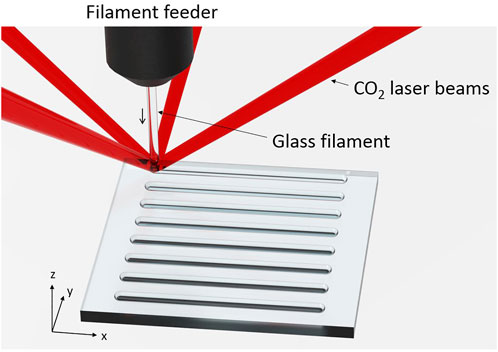
\includegraphics[width=0.8\linewidth]{kth2022_fig1.jpg}
  \caption{Filament-based glass 3D printing setup of Liu, Oriekhov and Fokine (KTH Royal Institute of Technology): a \SI{196}{\micro\metre} fused-silica filament is fed into a hot zone formed by four focused CO$_2$-laser beams above a fused-quartz build plate on a motion stage. Reproduced from \citet{kth2022bonding} (Frontiers in Materials, CC BY 4.0).}
  \label{fig:kth}
\end{figure}

\section{Open problems and research frontiers}
\label{sec:open}

This section states the unresolved technical problems of molten glass AM as explicit problem statements, each with the evidence from the corpus that motivates it, the physical mechanism, the current best mitigation and what a solution would have to demonstrate.

\subsection{Problem 1: Devitrification and phase purity}
\textbf{Statement.} Determine the composition-, temperature- and time-dependent crystallisation risk of glass held in the working range in crucibles, nozzles and multi-layer thermal cycles, and design process windows and feedstocks that guarantee an amorphous product.

\textbf{Evidence and mechanism.} Every silicate glass is metastable between its liquidus and \(\Tg\); nucleation and growth are fastest at intermediate viscosities (\(10^{4}\)--\(10^{7}\)\,dPa\,s), exactly where deposition happens. Crucible-fed printers hold tens of kilograms of glass at the working point for days to weeks (\SIrange{2}{3}{week} campaigns in G3DP2 \citep{inamura2018}), and every layer re-heats the layer below through the crystallisation range. Borosilicates are known to be prone to devitrification during extrusion \citep{klein2015}, and fused silica devitrifies to cristobalite above roughly \SI{1100}{\celsius} in the presence of alkali or moisture, so the laser-melted fused-silica routes operate above \SI{1900}{\celsius} for seconds and quench through the crystallisation range in milliseconds. The powder-bed papers report fully amorphous parts by XRD for soda-lime \citep{datsiou2021} and comparable XRD for DED deposits and substrate \citep{spirrett2023}; the crucible-fed papers report none. The absence of reported devitrification is therefore not evidence of its absence: soda-lime studio glasses are formulated for a long working range and low liquidus, and the risk will rise as the community moves to borosilicate, aluminosilicate and recycled compositions with contaminants.

\textbf{Required.} Time--temperature--transformation data for candidate compositions at the relevant heating rates; in-line detection (Raman or optical scattering) of early crystallisation; and nozzle designs that avoid stagnant, slowly cooled glass films on ceramic surfaces, which are the classic nucleation sites in glass forming.

\subsection{Problem 2: Optical transmittance, wavefront distortion, bubbles and layer-seam optics}
\textbf{Statement.} Quantify and then control the four optical defects of printed glass---bulk transmission loss, refractive-index inhomogeneity (striae), bubble entrapment and periodic surface relief at layer seams---to the level required for a stated application class (window, lens, waveguide).

\textbf{Evidence and mechanism.} No paper in the corpus reports a spectrophotometric transmission curve for a crucible-fed printed part; transparency is documented photographically and by caustic projection \citep{klein2015,inamura2018}. For laser-filament parts, transmittance and index homogeneity were measured for fused quartz \citep{luo2018quartz}, a transmitted-beam camera showed a homogeneous wavefront without bubbles or boundary layers in LGD specimens \citep{lgd2024homog}, and index homogeneity was compared with commercial optical glass only for the indirect DIW route \citep{destino2018}. Bubbles arise from three sources: gas dissolved in the melt released on reheating (``reboil'', observed spectroscopically above a threshold temperature \citep{luo2017heat}), gas trapped between an incoming filament and the previous layer when wetting is incomplete (the ``wiggly line'' regime \citep{kth2022bonding}), and inter-particle porosity in powder routes (\SI{12}{\percent} \citep{datsiou2021}). Striae arise from incomplete homogenisation of the melt in gravity-fed crucibles and from the thermal history difference between filament core and surface in laser routes. Layer seams act as cylindrical lenslets: a wall of \SI{10}{mm} cords is a periodic refractive surface that focuses light into caustics---attractive for art and lighting \citep{brun2017,commons_caustics} but fatal for imaging optics unless the faces are ground and polished, as was done for all mechanical and optical test samples \citep{klein2015,mit2024masonry}.

\textbf{Required.} Standardised reporting of transmission (\SIrange{400}{2000}{nm}), haze and transmitted wavefront error for printed coupons; a model linking seam relief amplitude to cord temperature, surface tension and dwell time (the visco-capillary healing time \(\eta a/\sigma\) of \cref{sec:physics}); and fining strategies (thermal soak, low-viscosity fining agents, vacuum) compatible with a printer crucible.

\subsection{Problem 3: Thermal shock, stress accumulation and polarimetric stress mapping}
\textbf{Statement.} Predict, measure and minimise the three-dimensional residual stress field of a printed glass part as a function of geometry, thermal architecture and annealing schedule, with a validated non-destructive measurement.

\textbf{Evidence and mechanism.} \Cref{eq:stress} shows that \SI{100}{\celsius} of through-thickness gradient during vitrification leaves \SI{40}{MPa} in soda-lime. Cold-printed G3DP samples had one fifth of the flexural strength of hot-printed ones and visible radial stress \citep{klein2015}; substrate cracking is the dominant failure of powder-fed DED on thin float glass \citep{spirrett2023}; and the coaxial LGD head exists because asymmetric heating of a fibre produced ``very high residual stress'' \citep{lgd2021coaxial}. Fused silica is forgiving; every other glass is not. Yet the only stress measurements in the corpus are qualitative polariscope readings \citep{klein2015} and an absence-of-birefringence statement \citep{kth2022bonding}. Photoelastic tomography and scattered-light polariscopy can deliver quantitative 3D stress in complex glass articles \citep{aben2008}, and a coupled thermo-mechanical phase-transformation framework has been proposed for glass AM, but no printed-glass study has yet combined a thermal-history model with a measured stress field.

\textbf{Required.} Thermo-viscoelastic simulation (structural relaxation with the Tool--Narayanaswamy--Moynihan model) of a multi-layer build; validation by scattered-light polariscopy on witness coupons printed alongside parts; and design rules for wall thickness and print time versus chamber temperature.

\subsection{Problem 4: Nozzle wear, chemical corrosion and seal lifetime above \SI{1200}{\celsius}}
\textbf{Statement.} Extend the continuous operating life of the glass-contact components of a molten extrusion printer beyond the two-to-three-week campaigns of alumina nozzles, and enable borosilicate and aluminosilicate processing at \SIrange{1250}{1400}{\celsius}.

\textbf{Evidence and mechanism.} Molten alkali silicates dissolve alumina and silica refractories by alkali diffusion into the glassy phase, exudation and pore formation; fused-cast AZS and high-zirconia refractories resist best but still wear and must be replaced \citep{zircorr2025}. Contact corrosion, not motion accuracy, set the campaign length of G3DP2 \citep{inamura2018}, and the crucible and refractory cost was an explicit target of the G3DP3 redesign \citep{mit2024masonry}. The glass industry's answer for fibre bushings and stirrers is platinum--rhodium (80/20 or 90/10) which operates to about \SI{1600}{\celsius} and, alloyed or dispersion-strengthened with zirconia, forms bushing nozzle tips \citep{pgm2010}; Corning's application specifies exactly this for an induction-heated printer crucible \citep{patent_corning2021}. The barriers are cost (a \SI{10}{mm} bore, \SI{50}{mm} long Pt--Rh nozzle is tens of grams of platinum-group metal), oxidation and volatilisation of rhodium above \SI{1200}{\celsius} in air, and thermal-expansion mismatch at the ceramic--metal joint. Sealing is the second problem: refractory mortar joints between crucible and nozzle, and fibreboard skirts between kiln and moving carriage, are consumables; the patent's shears and torch manifold add further wear parts.

\textbf{Required.} Life tests of candidate nozzle materials (Pt--Rh, Pt--Au dispersion alloys, iridium, dense zirconia, SiC-coated graphite under inert gas) in the specific glass; nozzle geometries that avoid stagnant films; and modular, quick-change nozzle cartridges. The laser processes avoid the problem by removing the nozzle, which is why the fused-silica market has gone to them.

\subsection{Problem 5: Closed-loop monitoring and real-time slump control}
\textbf{Statement.} Close the loop from measured cord geometry and temperature to feed rate, travel speed and heat input on the layer time scale, so that bead width, layer height and overhang stability are held to specification without operator intervention.

\textbf{Evidence and mechanism.} Crucible-fed printers currently control only temperatures and travel speed; flow drifts with head and nozzle wetting, and geometry errors accumulate at convexity changes \citep{klein2015,inamura2018}. G3DP3 corrects set points between prints by comparing printed and predicted mass \citep{stern2024cgc}---a batch, not a real-time, loop. Laser-filament processes have moved further: closed-loop melt-pool temperature from a pyrometer \citep{lgd2025tempctrl} and from a thermal camera on a deterministic real-time platform \citep{dgf2026control} are demonstrated, and the latter shows that multilayer walls are impossible without it. What is missing on all platforms is geometric feedback: a measurement of cord width and height (structured-light or laser-line profilometry through the chamber window, or thermal-image edge detection) and of slump (deviation of the top layer from the toolpath), converted into travel-speed and feed corrections. Metal DED has such controllers; glass adds the difficulties of a radiating, transparent, viscous cord in a \SI{500}{\celsius} chamber.

\textbf{Required.} A validated slump model (the sag-velocity scaling of \cref{sec:physics}) as the plant model; sensing of top-layer temperature and width at \(\ge\)\SI{10}{Hz}; and model-predictive control of travel speed and nozzle temperature with the annealing chamber as a slow disturbance.

\subsection{Problem 6: Interlayer bonding, anisotropy and mechanical qualification}
\textbf{Statement.} Establish statistically qualified mechanical properties of printed glass---including the anisotropy between along-layer and across-layer directions---sufficient for structural design codes.

\textbf{Evidence.} Klein et al.\ measured a \SI{40}{\percent} difference between orientations and \SI{60}{\percent} of material strength across layers with sample counts too small for statistics \citep{klein2015}; Inamura et al.\ reported \SIrange{41}{56}{MPa} on eight cylinders and adopted a safety factor of ten \citep{inamura2018}; the masonry study tested multiples of one design and found initial-fracture strengths from \SI{3.6}{MPa} (fully printed, thick base) to \SI{42}{MPa} and ultimate strengths of \SIrange{64}{118}{MPa}, with dimensional accuracy under \SI{1}{mm} \citep{mit2024masonry}. Powder-bed parts are an order of magnitude weaker \citep{datsiou2021}, and quartz DED reaches \SI{95}{\percent} of bulk \citep{lang2024}. Four-point bending on statistically meaningful populations, Weibull analysis, and fractography of layer interfaces are the missing elements, together with surface treatments (fire polishing, chemical strengthening) whose effect on printed glass was inconsistent \citep{inamura2018}.

\subsection{Problem 7: Feedstock chemistry and recycled glass}
\textbf{Statement.} Extend the material set beyond soda-lime studio glass to container and float cullet, borosilicate, aluminosilicate and specialty glasses while maintaining a stable process.

\textbf{Evidence.} Recycled container and float glass have been printed on G3DP3 after VFT-based viscosity matching, with \SI{295}{\celsius} working ranges nearly identical to studio glass; contamination sensitivity of post-consumer cullet was flagged as the next study \citep{stern2024cgc}. Maple Glass Printing draws its own cane from recycled cullet and must segregate colours \citep{maple_ammedia}. Borosilicate has been claimed by Micron3DP \citep{micron3dp_acers} and laser-deposited from rods \citep{froehlich2022}, but no crucible-fed borosilicate print with reported properties exists in the corpus; the required \SI{1270}{\celsius} working point (\cref{tab:vft}) exceeds current nozzle limits (Problem 4). Multi-material printing (dual crucibles, colour gradients from frit added to the melt \citep{klein2015}) and functionally graded glass are surveyed in a 2026 review \citep{multimat2026}. Molten lunar regolith extruded from a platinum--rhodium crucible under vacuum has been demonstrated as an in-situ resource utilisation route \citep{regolithreview2023,regolithvac2024}, and Evenline has stated a target of \SI{1700}{\celsius} operation for borosilicate, silica and regolith \citep{stern2024cgc}.

\subsection{Problem 8: Energy, cost and throughput}
\textbf{Statement.} Establish the unit economics of molten glass AM relative to casting, pressing and blowing at the batch sizes where geometric customisation has value.

\textbf{Evidence.} The G3DP2 thermal module consumes \SI{15}{kW} during printing at \SI{5.2}{kg/h}, i.e.\ about \SI{3}{kWh/kg} before annealing, compared with roughly \SI{1}{kWh/kg} for a modern container furnace; the cane-fed Maple machines consume a few hundred watts but at grams-per-minute rates \citep{inamura2018,maple_ammedia}. Capital costs are USD~45\,000 for a Maple~3 \citep{maple_aniwaa}, price on request for Nobula \citep{nobula_aniwaa}, and not disclosed for Evenline, which sells parts and services rather than machines \citep{evenline_web}. The masonry study argues that AM wins where every unit differs or where tooling for pressed or cast blocks cannot be amortised \citep{mit2024masonry}; no published study yet quantifies the crossover batch size. \Cref{sec:industry} returns to this.

\subsection{Problem 9: Toolpath optimisation of transparent deposited materials for target optical properties}
\label{sec:open:toolpath}
\textbf{Statement.} Given a fixed global shape and a specified optical response---a transmittance or haze map, a caustic image, a reflection or scattering signature, or a lens or waveguide function---compute the deposition toolpath of a molten-glass (or other transparent extrusion) process, i.e.\ cord layout, layer height, bead width, coiling pattern, travel-speed and temperature schedule and hence surface relief, such that the printed part realises the optical target within the geometric tolerance of the shape.

\textbf{Evidence and mechanism.} In every direct deposition route the optical response of the part is a function of the toolpath, because each cord is a cylindrical lenslet whose relief is set by bead width, layer height and the visco-capillary healing time \(\eta a/\sigma\) of the seam (\cref{sec:physics}), and because the sewing-machine instabilities of a falling viscous thread provide a catalogue of periodic surface patterns selected purely by the ratio of travel to extrusion speed \citep{brun2017}. The literature has so far recorded this dependence rather than designed with it. Klein et al.\ created caustic patterns by projecting light through G3DP prints and noted that the striations and bulges of the print texture give ``a high degree of control'' over the redirection of light \citep{klein2015,klein2015thesis}; the G3DP2 columns are described as architectural-scale lenses whose geometric variation ``can drive, limit or control light transmission, reflection and refraction'' \citep{inamura2018}, yet their geometry was optimised for load, with the caustics an emergent by-product; the accompanying \emph{Glass~II} design study stated the intention to ``reverse-engineer geometry based on designed light patterns'' as future work, for which no publication has followed \citep{inglessis2017glass2}. The two computational halves of the problem do exist in isolation. Forward simulation: Weber, Reinhart and Oxman validated Radiance photon mapping of geometrically complex printed glass against measurements \citep{weber2020photon}. Inverse simulation: Kassubeck et al.\ built a differentiable multi-spectral caustic renderer with a regulariser that uses the known deposited glass volume, in order to reconstruct the shape of laser-deposited glass from its caustic image as a process-control signal; they explicitly distinguish this ``shape from caustic'' task from the ``caustic from shape'' task of computational caustic design \citep{kassubeck2021caustics}. Caustic design itself is mature for milled or polished freeform surfaces---micro-facet and continuous-surface formulations \citep{papas2011caustics,kiser2013caustics,yue2014caustics}, optimal-transport formulations for high-contrast images \citep{schwartzburg2014caustics}, and differentiable-rendering formulations for extended light sources \citep{zhou2025caustics}---and the graphics community has likewise solved the design of projected images from perforated shells \citep{zhao2016lampshades}, light routing through printed light pipes \citep{willis2012printedoptics,pereira2014routing}, spatially varying translucency and subsurface scattering \citep{dong2010sss,papas2013translucent,elek2017scattering,brunton2018translucency,nagasawa2023translucency} and custom reflectance from fabricated microgeometry \citep{weyrich2009microgeometry}; all of these assume a fabrication process that reproduces a computed surface or voxel field, never the toolpath of a self-smoothing viscous cord. Toolpath optimisation for glass exists only with a mechanical objective: Chhadeh et al.\ showed on rod-fed soda-lime deposition that layer orientation and toolpath govern bending strength through the heat retained during deposition \citep{chhadeh2026toolpath}---the same heat-retention physics that governs seam healing and therefore optical relief. In the laser-filament routes, deposition parameters already act as optical design variables at the single-element scale: the focal length of each lens in a printed silica microlens array is set by the number of layers and the radius \citep{kth2024microlens}, deposited fibre spheres form micro-lens matrices \citep{rettschlag2020microlens}, the deposition path of a coreless fibre is the light path of a curved waveguide \citep{kranert2020waveguide}, and fibre-fed printing with temperature feedback yields spherical and aspherical germanate lenses \citep{hong2023germanate}. In the indirect direct-ink-writing route the toolpath literally encodes an optical field, the refractive-index profile of gradient-index glass, through inline ink mixing \citep{destino2018,dyllaspears2020grin}, and dedicated gradient toolpath generators with curvature-based velocity compensation have been published for it \citep{sage2026fermat}; but the variable is composition, not cord geometry, and the part is sintered and polished afterwards. Finally, for transparent polymer extrusion the toolpath--optics relation has been quantified as a scalar design-of-experiments problem: layer height, road width, raster angle, orientation, extrusion multiplier and speed against transmittance and translucency \citep{kumar2022transparency,kumar2024transparency,vochozka2024translucency,hamp2021transmittance,quero2021microfluidic}, against absorption and scattering coefficients when \emph{low} transparency is the target \citep{amendola2021diffuse}, and against birefringence \citep{ren2023anisotropy}; FDM lenses are tuned through nozzle diameter and raster angle \citep{blachowicz2021optical,heinrich2016optics,gao2023review} or made clear by coating over the layer relief \citep{rooney2024lenses}, and the direction of the printed cords has been used to engineer the reflection anisotropy of a surface \citep{anisotag2023}. No publication was found, in web, OpenAlex or Crossref searches, that closes the loop from a target optical response to the toolpath of a glass or transparent-extrusion process under a fixed shape envelope; the commercial lighting and art products of \cref{sec:industry} rely on the default layer-seam caustics.

\textbf{Required.} (i) A forward model of cord cross-section relief and its healing as a function of the toolpath variables (bead spacing, layer height, over- or under-extrusion, travel-speed modulation, coiling regime, non-planar layers), coupled to a differentiable ray or photon model of the kind already available \citep{weber2020photon,kassubeck2021caustics}. (ii) A toolpath parameterisation that spans the range from seam-free transparency (dense, fully healed cords, the glass analogue of the aligned-rectilinear, zero-cooling recipes of polymer printing) to prescribed refractive relief for caustics, diffusion or directional reflection, while respecting the molten-glass constraints of a single continuous path, nozzle-set layer height, slump and thermal history (Problems 3 and 5). (iii) An optimisation formulation---optimal transport or gradient descent on the differentiable objective---with these fabrication constraints, and a statement of the trade-off between optical target, shape tolerance and mechanical strength, since the toolpath now serves three objectives. (iv) Validation by transmitted-wavefront and caustic-image measurement on printed coupons, which would at the same time supply the geometric feedback signal that Problem 5 lacks.

\section{Academic landscape}
\label{sec:academic}

\subsection{Method of mapping}
Research groups were identified from the harvested corpus (author affiliations recorded by OpenAlex), from citation chains in the primary papers, and from targeted searches for the institutions named in the review brief. \Cref{tab:academic} lists every group with at least one peer-reviewed molten-glass or laser-glass deposition publication, together with groups in adjacent fields (indirect routes, cast-glass structures) that shape the direct-deposition agenda. Negative findings are reported explicitly: for several institutions named in the brief no molten-glass AM output could be located, and this is stated rather than inferred.

\subsection{Core groups in direct molten deposition}
\paragraph{MIT Mediated Matter Group (Neri Oxman) and successors.} The G3DP platforms were developed 2014--2018 by John Klein, Michael Stern, Giorgia Franchin (Padova), Markus Kayser, Chikara Inamura, Daniel Lizardo, Peter Houk (MIT Glass Lab), Shreya Dave and colleagues, in collaboration with the Department of Mechanical Engineering, the Wyss Institute and industry partners (Skutt, Smart Ceramics, Deltech, Spiral Arts, Corning for viscometry) \citep{klein2015,inamura2018,brun2017,oxman_platform,medialab_glass2}. The group filed the two foundational MIT patents \citep{patent_us10266442,patent_us9919510}. Its output includes the 2015 G3DP demonstrations exhibited at Cooper Hewitt, the three-metre Glass II columns for the 2017 Lexus ``Yet'' exhibition in Milan (video: \href{https://player.vimeo.com/video/211778198}{GLASS II}; event: \href{https://vimeo.com/215835768}{Lexus Design Event 2017}), and the process video \href{https://commons.wikimedia.org/wiki/File:Matter-glass-printer.webm}{GLASS (2015)} released under CC BY-SA \citep{video_glass1,video_glass2,video_lexus2017}. After the Mediated Matter Group closed, the work continued in the MIT Department of Mechanical Engineering under Kaitlyn Becker (Fabrication-Integrated Design Lab) with Daniel Massimino and Charlotte Folinus, in partnership with Evenline \citep{mit2024masonry,mitnews2024bricks}.

\paragraph{Missouri University of Science and Technology and University of Notre Dame (Edward Kinzel, Robert Landers, Douglas Bristow).} The most sustained academic programme in laser filament deposition: rod-fed CO$_2$ printing in 2014 \citep{luo2014jmse}, soda-lime filaments and the low-order melt-temperature model \citep{luo2017sodalime}, heat-transfer measurement by incandescence spectroscopy \citep{luo2017heat}, fused quartz optics \citep{luo2018quartz,luo2016spie}, SMF-28 fibre feedstock and free-standing structures \citep{hostetler2018fiber,hostetler2018sff,hostetler2019optics}, bubble-formation mechanisms \citep{bubbles2018}, side-injected interface heating \citep{capps2021interface}, hollow tubes \citep{dgf2023tubes}, an Elsevier book chapter defining ``digital glass forming'' \citep{kinzel2025dgf}, and thermal-camera closed-loop control with Los Alamos and Notre Dame co-authors \citep{dgf2026control}. Junjie Luo's 2017 dissertation collects the early work.

\paragraph{Laser Zentrum Hannover and Leibniz University Hannover (Stefan Kaierle, Ludger Overmeyer, Katharina Rettschlag, Khodor Sleiman, Peter J{\"a}schke).} The LGD process (2018), coaxial LGD with thermal simulation (2021), fused-silica fibre structural components (2022), the GROTESK collaborative research programme on optical, thermal and structural components \citep{grotesk2022}, and the 2024 homogeneity study with \SI{21}{nm} roughness \citep{witzendorff2018,lgd2021coaxial,lgd2022fibers,lgd2024homog}. Adjacent work at the Hannover laser cluster covers waveguide printing from coreless fibres and thermal modelling.

\paragraph{KTH Royal Institute of Technology (Michael Fokine, Chunxin Liu, Taras Oriekhov) and Nobula3D.} Systematic process mapping of filament-based fused-silica printing \citep{kth2022bonding}, silica microlens arrays \citep{kth2024microlens}, a 2022 doctoral thesis on additive manufacturing of fused silica glass, and the 2021 spin-off Nobula3D whose CEO is Chunxin Liu \citep{nobula_kthventures,nobula_fabbaloo}. Sustainable photonic-component fabrication by glass 3D printing is funded through the Swedish WISE materials programme. The Frontiers paper was edited by Stefan Karlsson of RISE Research Institutes of Sweden, which is the extent of RISE's traceable involvement in glass AM; RISE's Application Center for Additive Manufacturing in M{\"o}lndal is metal- and polymer-focused.

\paragraph{University of Nottingham, Centre for Additive Manufacturing (Ruth Goodridge, Kyriaki Corinna Datsiou, Fiona Spirrett, Ian Ashcroft; with Glass Technology Services).} L-PBF of soda-lime in a commercial machine \citep{datsiou2019}, parameter optimisation and property evaluation \citep{datsiou2021}, and powder-fed DED for bottle decoration \citep{spirrett2023}; Datsiou has since moved to Loughborough.

\paragraph{TU Ilmenau (Jean Pierre Bergmann, J{\"o}rg Hildebrand, Edda R{\"a}dlein) and Carl Zeiss Jena (Jens Bliedtner).} Rod-fed CO$_2$ laser deposition of borosilicate and soda-lime \citep{froehlich2022} and powder-bed laser processing of alkali borosilicate \citep{boro2025laser}.

\paragraph{TU Darmstadt (Jens Schneider, Matthias Seel) and the structural-glass community.} Fused glass deposition modelling of soda-lime rod on float glass \citep{seel2018}, printed glass point fixings \citep{pointfixings2024}, and thin-glass composite fa\c{c}ade panels at TU Dresden (Christian Louter, Daniel Pfarr) \citep{pfarr2023} that motivated Evenline's rib-on-plate printing.

\paragraph{Institute of Optics and Electronics, Chinese Academy of Sciences, Chengdu (Yuntao Cheng, Tao Xu).} Coaxial powder-fed DED of quartz glass with \SI{95}{\percent} of bulk strength \citep{lang2024} and PID closed-loop melt-pool temperature control with coaxial wire feeding \citep{lgd2025tempctrl}.

\paragraph{South China University of Technology and Clemson University (Jincheng Lei, Hai Xiao).} Paste extrusion with in-situ CO$_2$ laser melting of fused silica \citep{ieee2019dlm,paste2024}.

\paragraph{Lomonosov Moscow State University (Andrey Gusarov, Roman Khmyrov) and FH Aachen (Miranda Fateri, Andreas Gebhardt).} Early crack-free SLM of silica \citep{khmyrov2016,khmyrov2014} and SLM of soda-lime powder \citep{fateri2015}; Fudan University (Lingbao Kong) extended SLM to irregular powders \citep{slmirregular2023}, and the Chinese University of Hong Kong published the monolayer densification model \citep{slmsim2024}.

\paragraph{Universit\'e Laval, COPL (Youn\`es Messaddeq) and \L{}ukasiewicz Research Network / University of Warsaw (Przemys\l{}aw Go\l{}\k{e}biewski, Ryszard Buczy\'nski).} Direct melt extrusion of \emph{low-temperature} glasses: As$_{40}$S$_{60}$ chalcogenide filaments printed at \SI{140}{\celsius} above \(\Tg = \SI{188}{\celsius}\) on a modified commercial FDM printer \citep{baudet2019}, and pneumatic crucible extrusion of heavy-metal-oxide soft glass into 2500-rod photonic-crystal-fibre preforms that were drawn into single-mode fibre \citep{laval2023preform}. These are molten-deposition processes in every physical sense and are the natural bridge to specialty-fibre manufacturing. No molten-glass AM output from McGill University could be located; McGill's Additive Design and Manufacturing Laboratory works on metals and polymers.

\subsection{Adjacent groups that shape the field}
\paragraph{TU Delft, Glass \& Transparency Research Group (Faidra Oikonomopoulou, Telesilla Bristogianni).} Not a molten-deposition group, but the source of the cast-glass interlocking masonry designs (Block Type E, the figure-eight) that MIT/Evenline adapted for printing, of the 3D-printed sand-mould and lost-wax casting routes for complex glass, and of the topology-optimised cast-glass megalith studies that define the structural-glass application space \citep{mit2024masonry}; the group also hosted the Challenging Glass 9 conference (June 2024, Delft) where Evenline's recycled-glass paper appeared \citep{stern2024cgc}. Reports of a TU Delft--TU Darmstadt collaboration on extrusion of molten glass tracks could not be traced to a peer-reviewed source.

\paragraph{Karlsruhe Institute of Technology and University of Freiburg, NeptunLab (Bastian Rapp, Frederik Kotz-Helmer, Dorothea Helmer).} The indirect fused-silica route (Glassomer) \citep{kotz2017,mader2021}, micro-CAL with UC Berkeley \citep{toombs2022}, and the Elsevier reference book \citep{rappkotz2024book}; the benchmark against which direct routes are measured for resolution and surface finish.

\paragraph{Lawrence Livermore National Laboratory (Rebecca Dylla-Spears, Joel Destino, Du Nguyen, Nikola Dudukovic).} Direct ink writing of silica sols to optical-grade and gradient-index glass \citep{nguyen2017,destino2018,llnl2018}, and the sol-gel AM review with Creighton University \citep{solgel2025}. LLNL's work is indirect; the brief's mention of ``direct glass deposition'' at LLNL corresponds to its direct-ink-writing programme.

\paragraph{Fraunhofer institutes (IKTS, ISC, IPT, ILT).} Fraunhofer IKTS lists glasses among the materials it processes by powder-bed and suspension-based AM and Fraunhofer ILT leads in laser material deposition of metals, but no Fraunhofer publication on molten glass deposition surfaced in any query; the German centre of gravity for laser glass AM is the Hannover cluster (LZH, LUH) and Ilmenau/Jena.

\paragraph{Nagaoka University of Technology.} The Functional Glass Engineering Laboratory works on functional glasses and glass-ceramics (including solid-state sodium-ion battery electrolytes) and other laboratories use commercial polymer 3D printers, but no molten-glass AM publication from Nagaoka could be located in English or Japanese queries.

\paragraph{University of Utah (Rajesh Menon, Berardi Sensale-Rodriguez) with University of Galway and Queen's University Belfast.} The NSF-funded STELLAR project (USD~1.4\,M, 2025) develops femtosecond-laser fusion of glass powder with micrometre features over centimetre areas at reduced temperature for photonic sensors and nanosatellite optics \citep{utah2025}.

\paragraph{Deakin University / ANU / RMIT (Nick Birbilis, Jeffrey Sarmiento, Roland Snooks).} Authors of the 2025 critical review with emphasis on semi-solid processing and on architecture and art \citep{critical2025}; Birbilis is co-founder of Maple Glass Printing, linking the review to the commercial desktop route. Other recent reviews are \citet{zhang2021review,matdes2023review,micromachines2022,jmmp2026review,multimat2026}.

\subsection{Academic groups directory}
\begin{sidewaystable}[p]
  \centering\scriptsize
  \caption{Academic groups directory for molten and laser glass deposition (direct routes) and the adjacent indirect and structural-glass groups. DOIs are given for the key publication in the harvested corpus.}
  \label{tab:academic}
  \begin{tabular}{@{}L{2.9cm}L{2.5cm}L{2.8cm}L{2.9cm}L{4.2cm}L{4.2cm}@{}}
    \toprule
    Lab / group & Institution & Key PIs & Core machine / process & Notable contribution & Key publication DOI\\
    \midrule
    Mediated Matter Group & MIT Media Lab (2014--2020) & N.\ Oxman; J.\ Klein, M.\ Stern, C.\ Inamura, D.\ Lizardo, P.\ Houk & G3DP, G3DP2: crucible-fed molten soda-lime extrusion, 3-zone kilns, 4-axis bed & First transparent molten-glass printer; \SI{5.2}{kg/h}; 3 m Milan columns; two US patents & 10.1089/3dp.2015.0021; 10.1089/3dp.2018.0157\\
    Fabrication-Integrated Design Lab & MIT Mechanical Engineering & K.\ Becker; D.\ Massimino, C.\ Folinus (with Evenline) & G3DP3 (Evenline) & Interlocking recycled-glass masonry, 64--118 MPa ultimate; design rules for glass AM & 10.1007/s40940-024-00279-8\\
    Laser Precision Manufacturing Lab & Missouri S\&T \(\rightarrow\) Univ.\ of Notre Dame & E.\ C.\ Kinzel, R.\ G.\ Landers, D.\ A.\ Bristow; J.\ Luo, J.\ Hostetler, N.\ Capps & Digital glass forming: CO\(_2\)/CO laser, rod, filament and SMF-28 fibre feed, 4-axis stage & Melt-temperature model, spectroscopic monitoring, fused-quartz optics, thermal-camera closed loop (2026) & 10.1115/1.4035182; 10.1117/1.OE.57.4.041408; 10.1016/j.addma.2026.105306\\
    Laser Zentrum Hannover / LUH ITA & Hannover, Germany & S.\ Kaierle, L.\ Overmeyer, K.\ Rettschlag, K.\ Sleiman & Laser glass deposition (LGD), lateral and coaxial CO\(_2\) heads, quartz fibre & Crack-free quartz structures; coaxial LGD; \(R_a\) 21 nm as-printed & 10.1016/j.procir.2018.08.109; 10.1016/j.procir.2024.08.116\\
    Laser Physics / Fokine group & KTH Royal Institute of Technology, Stockholm & M.\ Fokine, C.\ Liu, T.\ Oriekhov & Direct glass laser deposition, four-beam CO\(_2\), \SI{196}{\micro\metre} F300 fibre & Bonding-width process map, 105-layer walls, microlens arrays \(R_a\) 0.12 nm; spin-off Nobula & 10.3389/fmats.2022.978861; 10.1089/3dp.2022.0112\\
    Centre for Additive Manufacturing & University of Nottingham & R.\ Goodridge, K.\ C.\ Datsiou, F.\ Spirrett, I.\ Ashcroft & L-PBF and powder-fed DED of soda-lime & Process window, 12\% porosity, 6.5 MPa; DED bottle decoration & 10.1111/jace.16440; 10.1016/j.addma.2021.101880; 10.1111/jace.18638\\
    Production Technology / Glass & TU Ilmenau; Carl Zeiss Jena & J.\ P.\ Bergmann, J.\ Hildebrand, E.\ R{\"a}dlein, J.\ Bliedtner & Rod-fed CO\(_2\) deposition; PBF-LB of borosilicate powder & Borosilicate and soda-lime rod deposition; PBF morphology map 38--94\% density & 10.1007/978-3-030-95463-5\_10; 10.3390/jmmp9090305\\
    Institute of Structural Mechanics and Design & TU Darmstadt; TU Dresden & J.\ Schneider, M.\ Seel; C.\ Louter, D.\ Pfarr & Fused glass deposition of rod on float glass & All-glass connections and point fixings; thin-glass composite fa\c{c}ades & 10.1002/mawe.201800075; 10.1007/s40940-024-00290-z\\
    Lightweight Optics \& Advanced Materials Center & IOE, Chinese Academy of Sciences, Chengdu & Y.\ Cheng, T.\ Xu, M.\ Lang, J.\ Chen & Coaxial powder- and wire-fed laser DED of quartz & 72 MPa quartz (95\% bulk); PID closed-loop melt-pool temperature & 10.1089/3dp.2022.0137; 10.3390/mi16010029\\
    Lei / Xiao groups & South China Univ.\ of Technology; Clemson & J.\ Lei, H.\ Xiao & Silica paste printing + in-situ CO\(_2\) laser melting & Transparent fused silica without furnace step & 10.1016/j.addma.2024.104135\\
    Laser processing / SLM groups & Lomonosov MSU; FH Aachen; Fudan; CUHK & A.\ Gusarov, R.\ Khmyrov; M.\ Fateri, A.\ Gebhardt; L.\ Kong; W.\ Zhang & SLM of silica and soda-lime powder; densification model & Crack-free silica beads; 93--95\% density; monolayer simulation & 10.1007/s00170-015-8051-9; 10.1111/ijac.12338; 10.1016/j.jmrt.2023.09.011\\
    COPL & Universit\'e Laval, Qu\'ebec & Y.\ Messaddeq, Y.\ Ledemi & Filament FDM of chalcogenide glass (\(\Tg\) 188 \si{\celsius}) & First 3D-printed chalcogenide glass; IR optics, fibre preforms & 10.1364/OME.9.002307\\
    Glass Dept.\ / Photonics & \L{}ukasiewicz Research Network; Univ.\ of Warsaw & P.\ Go\l{}\k{e}biewski, R.\ Buczy\'nski & Pneumatic crucible extrusion of soft glass rods & 2500-rod printed PCF preform drawn to single-mode fibre & 10.1016/j.addma.2023.103899\\
    \midrule
    Glass \& Transparency Research Group & TU Delft & F.\ Oikonomopoulou, T.\ Bristogianni & Cast glass; 3D-printed sand and wax moulds; interlocking masonry & Structural cast-glass masonry designs adopted for glass AM; Challenging Glass conference & (design source cited in 10.1007/s40940-024-00279-8)\\
    NeptunLab & Univ.\ of Freiburg / KIT & B.\ E.\ Rapp, F.\ Kotz-Helmer, D.\ Helmer & Indirect: silica nanocomposite SLA, FDM/FFD, micro-CAL; Glassomer & Transparent fused silica by photopolymer routes; reference book & 10.1038/nature22061; 10.1002/advs.202103180; 10.1126/science.abm6459\\
    Materials Science / Optics & Lawrence Livermore National Laboratory; Creighton & R.\ Dylla-Spears, J.\ Destino, D.\ Nguyen & Indirect: direct ink writing of silica sols & Optical-grade and gradient-index printed glass & 10.1002/adma.201701181; 10.1002/admt.201700323\\
    STELLAR project & Univ.\ of Utah; Univ.\ of Galway; Queen's Belfast & R.\ Menon, B.\ Sensale-Rodriguez & Femtosecond-laser fusion of glass powder & \SI{1}{\micro\metre} features at reduced temperature (NSF, 2025) & (web) \\
    Review authors & Deakin / ANU / RMIT; Zhejiang; CUG Wuhan & N.\ Birbilis; J.\ Qiu; L.\ Hao & --- & Critical and comprehensive reviews 2020--2026 & 10.3390/app15063414; 10.1007/s12200-020-1009-z; 10.1016/j.matdes.2023.111736\\
    \bottomrule
  \end{tabular}
\end{sidewaystable}

\section{Industrial landscape, spin-offs and applications}
\label{sec:industry}

\subsection{Overview}
Commercial molten glass AM in 2026 consists of three small companies that build or operate molten-deposition machines (Evenline, Maple Glass Printing, Nobula3D), one that pioneered the field and went quiet (Micron3DP), one abandoned corporate patent filing (Corning), several indirect-route companies that compete for the same optics and microfluidics customers (Glassomer and the binder-jetting start-up Vitriform3D), and a small number of research-service arrangements (Mo-Sci with Northwestern, the RIT--Evenline partnership). No public company sells a molten glass printer; total disclosed external funding across the direct-route firms is below EUR~5 million. \Cref{tab:industry} gives the directory; the text below profiles each entity and then discusses application verticals and unit economics.

\begin{figure}[htbp]
  \centering
  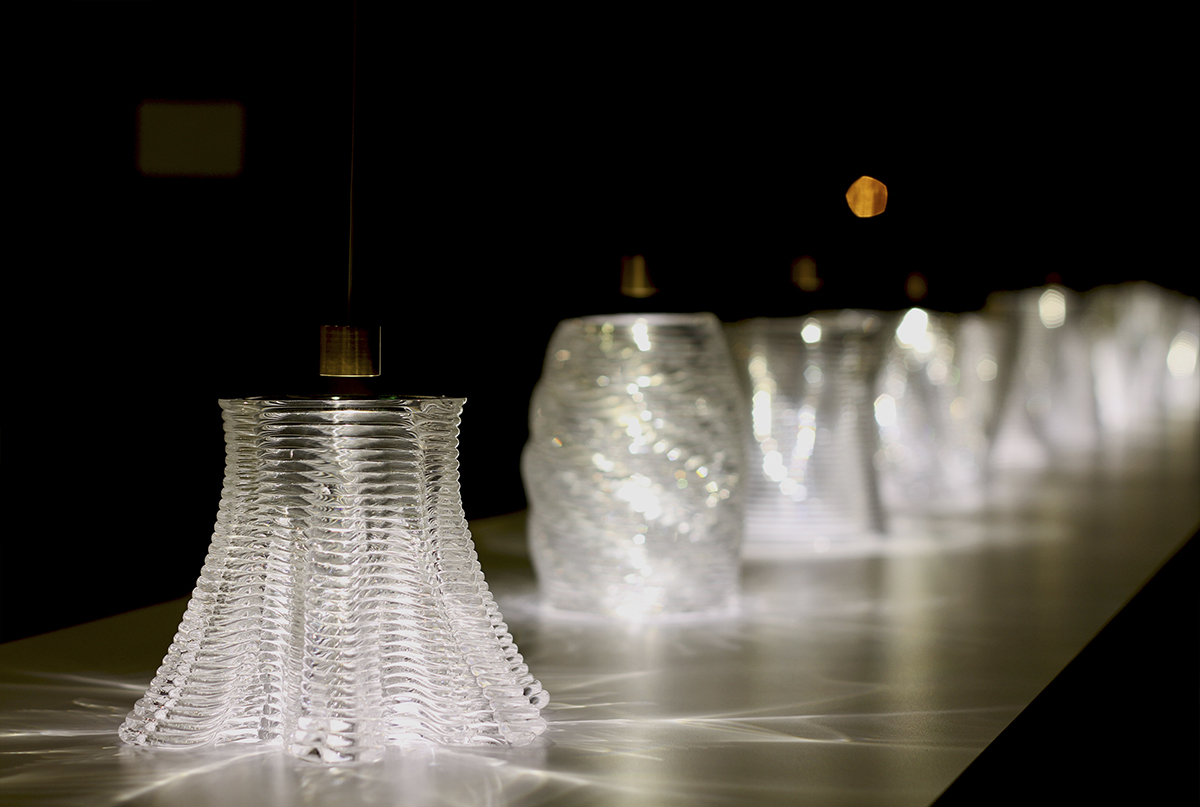
\includegraphics[width=0.8\linewidth]{commons_caustics.jpg}
  \caption{Printed soda-lime glass lamps from the MIT G3DP platform, illuminated from above; the periodic relief of the \SI{10}{mm} cords acts as an array of cylindrical lenslets and projects caustic patterns onto the table. The image illustrates both the optical signature of layer seams (\cref{sec:open}, Problem 2) and the lighting and art market that has been the first commercial outlet for molten glass AM. Photograph: Neri Oxman, Wikimedia Commons, CC BY-SA 4.0 \citep{commons_caustics}.}
  \label{fig:caustics}
\end{figure}

\subsection{Company profiles}
\paragraph{Evenline Inc.\ (Rochester, New York, USA).} Founded by Michael Stern, co-inventor of G3DP and G3DP2 at MIT and formerly of MIT Lincoln Laboratory, Evenline owns and operates the G3DP2 and the third-generation G3DP3 (``3D Glass Printer Mark III'') and sells printed art, lighting and design objects, custom parts for clients, and research services rather than machines \citep{evenline_web,acers2024recent,threednatives2025}. The G3DP3 prints \qtyproduct{325 x 325 x 380}{mm} from studio, container and float soda-lime glass at up to \SI{1200}{\celsius} with infrared thermographic calibration \citep{mit2024masonry,stern2024cgc}. The company hosted its printer at the Rochester Institute of Technology's College of Art and Design in 2023, where Stern teaches a digital-glass elective and where recycled bottle glass melted at \SI{2300}{\degree}F (\SI{1260}{\celsius}) is upcycled into printed objects; collaborations with NASA and DARPA on molten processing of lunar regolith are cited, and a Kickstarter campaign supported the recycled-glass programme \citep{rit2023}. With MIT it produced the interlocking masonry study \citep{mit2024masonry,mitnews2024bricks} and the recycled float and container glass study \citep{stern2024cgc}, and it stated that a next-generation G3DP4 could be a wide, low chamber for printing on large float sheets or a \SI{1700}{\celsius} machine for borosilicate, silica and regolith \citep{stern2024cgc}. Stern and Lizardo also founded Lios Design for printed architectural lighting. Intellectual property rests on the two MIT patents \citep{patent_us9919510,patent_us10464305,patent_us10266442}; funding is undisclosed.

\paragraph{Maple Glass Printing Pty Ltd (Melbourne, Australia).} Founded in 2017 by materials engineers Nick Birbilis and Darren Feenstra from Monash University; left university laboratories for its own premises in 2020, received a patent filing and commercialisation grant funding in late 2020 and a Canberra Innovation Network ICON grant, and introduced the Maple~2 and Maple~3 as its first commercial machines in 2022--2023 \citep{monash_maple,maple_ammedia,maple_aniwaa}. The Maple~3 (\qtyproduct{170 x 200 x 300}{mm}, cane feed, \SI{1000}{\celsius} nozzle, \SI{1.5}{mm} nozzle, \SI{0.1}{mm} minimum layer, approximately USD~45\,000) and the Maple~4 (2025, \qtyproduct{200 x 200 x 300}{mm}, \SI{100}{kg}, single-phase mains, one-click printing, automatic mesh levelling, magnetic bed) are sold to universities, studios and laboratories; the Vitri-Glass cane machine closes the loop from cullet \citep{maple_ammedia,threednatives2025,maple_web}. Applications cited are art and demonstration pieces, laboratory implements for neon and fibre-optic research, an architectural display project with Foster + Partners using recycled glass, and, in development, large-format robotic-arm printing for windows and fa\c{c}ades combined with wire-arc additive manufacturing \citep{maple_ammedia}. Process videos are on the company's YouTube channel, including a Formnext 2023 demonstration \citep{maple_youtube}. Birbilis co-authored the 2025 critical review \citep{critical2025}.

\paragraph{Nobula3D AB (Stockholm, Sweden).} A 2021 KTH spin-off from Michael Fokine's group, led by CEO Chunxin Liu, offering a complete system of desktop printer, fused-silica filament and software based on direct glass laser deposition (DGLD) \citep{nobula_kthventures,nobula_fabbaloo}. Specifications: non-contact CO$_2$-laser heating to \SI{2200}{\celsius}, \qtyproduct{180 x 180 x 100}{mm} build volume, \SI{0.1}{mm} Z resolution, \SIrange{100}{250}{\micro\metre} feature resolution, print speed up to \SI{200}{mm/s}, \qtyproduct{1000 x 400 x 600}{mm} footprint, \SI{50}{kg}, price on request \citep{nobula_aniwaa,threednatives2025}. Target applications are microlenses, microfluidics, lab-on-a-chip and organ-on-a-chip devices, fibre optics and art; the company markets ``precision hardware, software, computer vision and optical-grade glass'' \citep{nobula_web}. Backers include KTH Holding, the STING incubator and the European Innovation Council, with a EUR~2.5 million EIC Accelerator grant reported \citep{nobula_kthventures}.

\paragraph{Micron3DP Ltd (Kfar Saba / Hod Hasharon, Israel).} Founded by Eran Gal-Or, an extruder specialist, and the first company to show molten glass printing publicly in mid-2015 (soft glass at \SI{850}{\celsius}, borosilicate at a claimed \SI{1640}{\celsius}, \SI{100}{\micro\metre} layers, later a \qtyproduct{200 x 200 x 300}{mm} build volume) \citep{micron3dp_acers,micron3dp_3dprint2017}. Alpha units were installed in-house in 2017 and again reported in 2021 with plans for external beta testing; Gal-Or co-authored a glass-microfluidics paper with the University of Helsinki \citep{microfluidics2019}. No product release, funding round or activity after 2021 could be found; the company is listed as seeking a strategic investor. Its patent-pending extruder details were never published.

\paragraph{Corning Incorporated.} Corning's 2016 application for an induction-heated 80/20 platinum--rhodium barrel-and-nozzle crucible fed with glass rods, extruding beads onto a platform, is the only large-glass-company filing on molten extrusion AM in the corpus; it was published in 2021 and abandoned \citep{patent_corning2021}. Corning's contribution to the field is otherwise as the viscometry partner of the first G3DP paper \citep{klein2015} and as the supplier of the boro-aluminosilicate substrates that define one of the four viscosity curves in \cref{fig:vft}.

\paragraph{Glassomer GmbH (Freiburg, Germany).} Founded in April 2018 as a KIT spin-off by Bastian Rapp, Frederik Kotz and Dorothea Helmer, Glassomer sells silica-nanocomposite resins and granulates for SLA, FDM and injection moulding, and a printing service, converting parts to fused silica by debinding and sintering at about \SI{1300}{\celsius} \citep{glassomer_interview,kotz2017,mader2021}. Reported funding is about USD~0.8 million from EU programmes (EIC, Horizon 2020, ATTRACT) and prize money \citep{glassomer_crunchbase}. It is the reference competitor for the small-part optics and microfluidics market that Nobula targets with the direct route.

\paragraph{Vitriform3D (Knoxville, Tennessee, USA).} Founded by University of Tennessee students Alex Stiles and Dustin Gilmer, selected for the DOE Innovation Crossroads programme in 2022, and partnered with Oak Ridge National Laboratory's Manufacturing Demonstration Facility: robotic binder jetting of \SIrange{90}{95}{\percent} recycled glass powder with \SIrange{5}{10}{\percent} polymer binder, oven-set, for tiles, coasters, signs and, in development, building cladding \citep{ornl2026}. It is not a molten route but competes directly with Evenline and Maple in the recycled-glass architectural niche.

\paragraph{Research-service and development entities.} Mo-Sci LLC (Rolla, Missouri) is developing, with Northwestern University, a 3D printing method for soda-lime, borosilicate and sealing glasses for high-temperature components \citep{mosci_web}. MIT Lincoln Laboratory announced a \SI{250}{\celsius} direct-ink-writing route in 2022 \citep{acers2024recent}. The University of Utah's STELLAR project is an academic--industrial consortium rather than a company \citep{utah2025}.

\subsection{Application verticals}
\paragraph{Architecture and fa\c{c}ades.} This is the vertical in which molten deposition has a unique position because only the crucible-fed route reaches masonry scale. The Milan columns (2017) demonstrated free-standing structural glass at \SI{3}{m} with a design strength of \SI{4.1}{MPa} at a safety factor of ten \citep{inamura2018}; the 2024 masonry study demonstrated full-size interlocking units with ultimate strengths of \SIrange{64}{118}{MPa}, dimensional accuracy under \SI{1}{mm}, and a fully hollow design ready for implementation \citep{mit2024masonry}; and rib-on-plate printing directly onto \SIrange{3.2}{9.5}{mm} float glass, including coated products, showed a path to stiffened transparent panels \citep{stern2024cgc}. Structural qualification (Problem 6) and fire and impact performance remain open, as does the circular-economy claim, which is credible because the masonry units are adhesive-free and remeltable.

\paragraph{Custom optics and lenses.} Laser-filament printing produces fused-silica lenses, microlens arrays with \SI{0.12}{nm} roughness and cylindrical-convex elements \citep{kth2024microlens,luo2018quartz}, waveguides and free-standing fibre from SMF-28 \citep{hostetler2018sff}; the LGD homogeneity work targets optical, thermal and structural components \citep{lgd2024homog,grotesk2022}. For imaging-grade bulk optics the indirect routes currently lead on index homogeneity \citep{destino2018}, and the direct routes compete on speed and on the absence of shrinkage.

\paragraph{Hermetic microfluidics and chemical reactors.} Glass microfluidics printed by the indirect route have been used for on-line mass-spectrometric reaction monitoring \citep{microfluidics2019}, and L-PBF parts, although opaque, are proposed for continuous-flow reactors and structured catalysts where chemical inertness outweighs transparency \citep{datsiou2021}. Nobula and Glassomer both target lab-on-a-chip devices. Direct laser-filament printing of sealed channels remains a research topic; hollow tubes have been printed \citep{dgf2023tubes}.

\paragraph{Packaging and luxury goods.} Powder-fed DED of soda-lime onto bottles offers one-step decoration without moulds \citep{spirrett2023}; a 2026 review of packaging glasses situates such customisation within container-glass sustainability \citep{packaging2026}. Evenline's printed spiral vessels with designer Josh Owen and its commissioned awards are the luxury-object end of the same market \citep{threednatives2025}.

\paragraph{Nuclear waste vitrification and high-temperature vessels.} No molten glass AM work for vitrification was found; the relevance is indirect---the Fluegel viscosity model underlying process calibration was built partly on nuclear-waste glass data \citep{fluegel2007}, and the platinum--rhodium crucible technology of vitrification melters is what a high-temperature printer nozzle would borrow \citep{pgm2010}. Mo-Sci's sealing-glass development addresses high-temperature hermetic components \citep{mosci_web}.

\paragraph{Space and in-situ resource utilisation.} Molten lunar regolith simulant extruded from a platinum--rhodium crucible under vacuum, and laser-fused regolith glass-ceramics, are active research lines that reuse molten-glass printer architectures \citep{regolithreview2023,regolithvac2024}; Evenline cites NASA and DARPA collaborations \citep{rit2023}.

\paragraph{Art, lighting and design.} The first and still largest revenue stream: Evenline's studio production, Maple's artist customers, and Nobula's ``arts'' listing. The optical signature of layer seams (\cref{fig:caustics}) is an asset here.

\subsection{Unit economics and business cases}
The available data permit only order-of-magnitude statements, which are nevertheless informative.

\emph{Capital cost.} A cane-fed desktop machine is USD~45\,000 \citep{maple_aniwaa}; a laser-filament desktop machine is priced on request but built from a \SI{25}{W} CO$_2$ laser, a fibre feeder and a small motion stage \citep{kth2022bonding,nobula_aniwaa}; a crucible-fed architectural machine is a \SI{19}{kW} thermal module with custom cast-alumina crucible, three kilns, a four-axis CNC and an annealing lehr \citep{inamura2018}---a six-figure build that no vendor sells.

\emph{Operating cost.} Energy is \SI{15}{kW} at \SI{5.2}{kg/h} (about \SI{3}{kWh/kg}) for G3DP2 plus annealing, versus roughly \SI{1}{kWh/kg} for industrial container furnaces; the crucible and refractories are consumables on a weeks-to-months cycle \citep{inamura2018,mit2024masonry}. Cane-fed machines use hundreds of watts but at gram-per-minute rates, so the energy per kilogram is comparable or higher; the cane itself must be drawn from cullet at additional cost \citep{maple_ammedia}. Laser processes deposit millilitres per hour and are viable only for small, high-value parts.

\emph{Material yield.} Molten deposition is near-net-shape with no mould and no sprue; losses are the lead-in and lead-out layers (cut off and remelted) and the crucible heel. Evaporative loss in laser printing is within measurement error (\SI{-1.6 +- 2}{\percent}) \citep{kth2022bonding}. Compared with kiln casting into 3D-printed sand moulds, AM eliminates the disposable mould but adds hours of machine time per unit.

\emph{Batch viability.} The masonry study's argument is the general one for AM: printing wins where every unit differs (topology-optimised or site-specific fa\c{c}ade elements) or where the tooling for pressing and casting cannot be amortised, and it loses to pressed glass block for identical units in volume \citep{mit2024masonry}. With a G3DP3 cycle of roughly one hour per double-height unit plus annealing, a single machine yields of the order of \(10^{3}\) masonry units per year---sufficient for demonstration walls and bespoke fa\c{c}ades, not for building stock. The crossover batch size has not been published by any group and is identified as an open question (\cref{sec:open}, Problem 8).

\subsection{Industrial systems directory}
\begin{sidewaystable}[p]
  \centering\scriptsize
  \caption{Industrial systems directory: molten-deposition machines and the principal indirect-route competitors. Temperatures are the maximum glass-processing temperature stated by the company or in the cited literature.}
  \label{tab:industry}
  \begin{tabular}{@{}L{2.6cm}L{2.7cm}L{3.2cm}L{2.3cm}L{3.4cm}L{3.6cm}L{2.2cm}@{}}
    \toprule
    Company (location, founded) & Machine name & Material compatibility & Max extruder / process temp. & Target market & Commercial status (2026) & Refs.\\
    \midrule
    Evenline Inc.\ (Rochester NY, USA; MIT spin-off, M.\ Stern) & G3DP2; G3DP3 ``3D Glass Printer Mark III'' (\qtyproduct{325 x 325 x 380}{mm}) & Studio, container and float soda-lime glass, incl.\ recycled cullet; colour by frit & \SI{1200}{\celsius} extrusion; furnace to \SI{1260}{\celsius} & Art, lighting, design objects; architectural masonry and fa\c{c}ade prototypes; custom parts; research (NASA, DARPA, RIT) & Operating; sells parts and services, not machines; G3DP4 planned & \citep{evenline_web,mit2024masonry,stern2024cgc,rit2023}\\
    Maple Glass Printing (Melbourne, Australia; 2017, N.\ Birbilis, D.\ Feenstra) & Maple 2, Maple 3 (\qtyproduct{170 x 200 x 300}{mm}), Maple 4 (\qtyproduct{200 x 200 x 300}{mm}); Vitri-Glass cane machine & Soda-lime cane, incl.\ recycled; colours segregated & \(\approx\)\SI{1000}{\celsius} nozzle & Education, art studios, laboratories (neon, fibre optics), architecture demonstrators & Machines on sale (Maple 3 approx.\ USD 45\,000); Maple 4 launched 2025; large-format robotic system in development & \citep{maple_ammedia,maple_aniwaa,threednatives2025,monash_maple}\\
    Nobula3D AB (Stockholm, Sweden; 2021, KTH spin-off, CEO C.\ Liu) & Nobula glass 3D printer (DGLD; \qtyproduct{180 x 180 x 100}{mm}) & Fused-silica filament (Nobula filament); silica glass & \SI{2200}{\celsius} (CO\(_2\) laser, non-contact) & Micro-optics, microfluidics, lab-/organ-on-a-chip, fibre optics, art & Available on request; EIC Accelerator EUR 2.5 M; KTH Holding, STING & \citep{nobula_aniwaa,nobula_fabbaloo,nobula_kthventures,nobula_web}\\
    Micron3DP Ltd (Kfar Saba, Israel; 2015, E.\ Gal-Or) & Unnamed high-resolution glass printer (\qtyproduct{200 x 200 x 300}{mm}, \SI{100}{\micro\metre} layers) & Soda-lime; borosilicate (claimed) & \SI{850}{\celsius} soft glass; \SI{1640}{\celsius} borosilicate (claimed) & Microfluidics, healthcare, architecture, art & Alpha units 2017--2021; no product; seeking investor; no activity found after 2021 & \citep{micron3dp_acers,micron3dp_3dprint2017,microfluidics2019}\\
    Corning Incorporated (Corning NY, USA) & Patent application only: induction-heated Pt--Rh crucible/nozzle, rod feed & Silicate glasses as rods \(\ge\)\SI{1}{mm} & n.r.\ (Pt--Rh to \(\sim\)\SI{1600}{\celsius}) & Glass articles (generic) & Application published 2021, abandoned & \citep{patent_corning2021}\\
    \midrule
    Glassomer GmbH (Freiburg, Germany; 2018, KIT spin-off) & Materials for open SLA/FDM printers; printing and injection-moulding service & Fused silica (nanocomposite \(\to\) sinter) & Sintering \(\approx\)\SI{1300}{\celsius} (indirect) & Optics, microfluidics, medical, automotive & Operating; approx.\ USD 0.8 M grants and prizes & \citep{glassomer_interview,glassomer_crunchbase,kotz2017}\\
    Vitriform3D (Knoxville TN, USA; 2022 DOE Innovation Crossroads) & Robotic binder jetting of recycled glass powder & 90--95\% recycled glass + 5--10\% binder & Oven-set (indirect) & Tiles, coasters, signage; building cladding in development & Start-up with ORNL/MDF support & \citep{ornl2026}\\
    Mo-Sci LLC with Northwestern University (Rolla MO, USA) & Development programme & Soda-lime, borosilicate, sealing glasses & n.r. & High-temperature components, hermetic seals & R\&D & \citep{mosci_web}\\
    MIT Lincoln Laboratory (Lexington MA, USA) & Direct-ink-writing route, \(\le\)\SI{250}{\celsius} & Silicate solution + inorganic nanoparticles & \SI{250}{\celsius} (indirect) & Thermally stable structures & Research announcement 2022 & \citep{acers2024recent}\\
    \bottomrule
  \end{tabular}
\end{sidewaystable}

\section{Future outlook and roadmap}
\label{sec:outlook}

\subsection{Where the field stands}
Ten years after the first automated molten glass printers, the direct route has split into two mature but disjoint capabilities. Crucible-fed extrusion produces architectural-scale, transparent soda-lime objects at kilograms per hour with bead-scale resolution and has crossed from laboratory to a small studio-manufacturing business with a credible circular-materials story \citep{inamura2018,mit2024masonry,stern2024cgc}. Laser-filament deposition produces fused-silica optics and micro-components at millilitres per hour with nanometre surfaces and has crossed into a first commercial desktop product and the first real-time controlled process \citep{lgd2024homog,kth2024microlens,nobula_aniwaa,dgf2026control}. Between them lies unoccupied territory: no process prints transparent borosilicate or aluminosilicate at centimetre scale, no crucible-fed machine has real-time geometric control, no laser process exceeds a few cubic centimetres per hour, and no printed glass part of any kind has a published Weibull strength distribution or a quantitative three-dimensional residual-stress map. The roadmap below is organised around closing these gaps and is stated as a sequence of milestones that the evidence suggests are reachable within roughly five years.

\subsection{Near-term milestones (1--2 years)}
\begin{enumerate}[leftmargin=*,itemsep=2pt]
  \item \textbf{Geometric closed-loop control on crucible-fed printers.} Thermal imaging is already on G3DP3 \citep{stern2024cgc}; adding bead-width extraction from the thermal image and a slump observer based on the sag-velocity scaling of \cref{sec:physics} would convert the present between-print mass correction into within-layer travel-speed control. The 2026 digital-glass-forming controller shows the architecture (deterministic real-time platform, camera in the loop) \citep{dgf2026control}.
  \item \textbf{Standardised optical and mechanical reporting.} A minimal coupon set---polished-face spectral transmission, transmitted wavefront, scattered-light polariscopy, four-point bending with Weibull statistics in two orientations---printed alongside every published part would make the modalities comparable. The tools exist \citep{aben2008,inamura2018}; the practice does not.
  \item \textbf{Recycled-glass qualification.} The viscosity-matching workflow \citep{stern2024cgc} should be extended to contaminated post-consumer cullet with a defined contamination tolerance, and the powder route's finding that irregular milled powder is processable \citep{slmirregular2023} should be tested for laser-filament feedstock drawn from cullet.
  \item \textbf{Fused-silica part scale-up.} The LGD and DGLD groups have shown fully dense walls of tens of millimetres \citep{lgd2024homog,kth2022bonding}; multi-fibre or rod feeding with side-injected heating \citep{capps2021interface} and coaxial ring beams \citep{lgd2021coaxial} are the identified levers to raise deposition rate by an order of magnitude without losing the \SI{20}{nm} surface.
\end{enumerate}

\subsection{Medium-term milestones (3--5 years)}
\begin{enumerate}[leftmargin=*,itemsep=2pt]
  \item \textbf{Borosilicate and aluminosilicate melt extrusion.} Requires a \SIrange{1300}{1450}{\celsius} melter and a nozzle that survives it. The candidates are platinum--rhodium (the Corning application and the fibre-bushing precedent \citep{patent_corning2021,pgm2010}) and dense zirconia; the barrier is cost and rhodium volatilisation. A quick-change platinum-alloy nozzle cartridge of tens of grams, with an inert-gas shroud, is a realistic engineering target and would unlock chemically resistant labware and low-expansion architectural glass. Evenline's stated \SI{1700}{\celsius} G3DP4 variant is the first public commitment \citep{stern2024cgc}.
  \item \textbf{Flow start--stop and multi-nozzle heads.} The MIT patents anticipate shears and multi-orifice nozzles \citep{patent_us9919510}; implementing them lifts the single-continuous-path constraint that currently dictates part design \citep{mit2024masonry} and enables dual-crucible multi-material printing, which the 2026 multi-material review identifies as the frontier \citep{multimat2026}.
  \item \textbf{Hybrid architecture: molten extrusion with laser surface conditioning.} A CO$_2$ laser tracking the nozzle could fire-polish the outer seam while it is still above the softening point, reducing the layer relief that limits optical use, and could locally reheat the previous layer for bonding on cold-chamber machines. Both are routine in polymer and metal directed energy deposition and have no glass-specific obstacle beyond chamber optics.
  \item \textbf{Validated thermo-mechanical simulation.} Coupling a layer-by-layer thermal model (the lumped and conduction models of \cref{sec:physics} are sufficient for soda-lime cords; laser melt pools need the Marangoni-resolved models now appearing \citep{machines2026meltpool,lgd2021coaxial}) to structural relaxation would let the annealing schedule be computed rather than inherited from studio practice, and would give the first predicted residual-stress fields to compare with photoelastic tomography.
  \item \textbf{Structural certification of printed masonry.} A test programme of the scale used for cast-glass masonry at TU Delft, applied to fully hollow printed units, with fire, impact and weathering, would move the 2024 feasibility result \citep{mit2024masonry} into a code-compliant product. This is the shortest path to a building-scale reference project.
\end{enumerate}

\subsection{Longer-term directions}
\emph{Large-format robotic deposition.} Maple's robotic-arm development and Evenline's wide-chamber concept both point to gantry- or arm-mounted heads for fa\c{c}ade panels; the physics favours printing onto preheated float sheet, which supplies the annealing mass and the optical face \citep{stern2024cgc,maple_ammedia}. The chamber then becomes a lehr that travels with the part.

\emph{Programmable optics from instabilities.} The coiling regime of the fluid-mechanical sewing machine \citep{brun2017} and the caustic design methods already applied to printed lamps suggest glass elements whose light distribution is programmed through deposition parameters rather than post-machining---a market that no other material can enter.

\emph{Direct fibre and preform manufacture.} Printed photonic-crystal-fibre preforms drawn to single-mode fibre \citep{laval2023preform} and free-standing fibre printed from SMF-28 \citep{hostetler2018sff} indicate a route from printer to fibre tower that bypasses stack-and-draw; specialty-fibre and chalcogenide IR optics \citep{baudet2019} are the first products.

\emph{Off-world construction.} Molten regolith extrusion from platinum--rhodium crucibles under vacuum \citep{regolithreview2023,regolithvac2024} is a molten-glass printer by another name; the nozzle-corrosion, devitrification and thermal-stress problems of this review are exactly its problems, with the added constraint of solar or laser heating.

\emph{Energy and circularity as the selling proposition.} Remelting cullet consumes less energy than melting virgin batch, printing eliminates moulds, and adhesive-free interlocking units are remeltable at end of life \citep{stern2024cgc,mit2024masonry}. If the crossover batch size (Problem 8) can be shown to be in the tens to hundreds of units for fa\c{c}ade elements, molten glass AM has a business case independent of art and lighting.

\subsection{Recommendations for research funders and practitioners}
\begin{itemize}[leftmargin=*,itemsep=1pt]
  \item Fund the instrumentation gap, not another demonstrator: quantitative stress, transmission and strength characterisation of printed glass is cheaper than a new machine and is what every downstream application needs.
  \item Treat nozzle and crucible corrosion as the critical-path materials problem for melt extrusion; a platinum-alloy or zirconia nozzle life test in three glasses is a well-posed, one-year project.
  \item Connect the two communities: the laser groups have control theory and optics, the extrusion groups have scale and materials handling; a laser-conditioned extrusion head is the natural joint project.
  \item Publish process windows in dimensionless form (Ohnesorge, visco-capillary time, energy density, \(\Delta T\) across the transformation range) so that results transfer between glasses and machines.
  \item Establish a shared benchmark part (a thin wall, a lens blank, a masonry-scale hollow) and report the coupon set above for every new process paper.
\end{itemize}

\subsection{Closing statement}
Molten hot glass AM has reached the point at which the remaining obstacles are engineering and metrology rather than feasibility. The physics is understood well enough to be written down in a page of equations; the machines exist in two complementary forms; the first products are sold. What separates the field from industrial adoption is the absence of quantitative process--property data, the corrosion-limited temperature ceiling of contact extrusion, and the lack of real-time geometric control. Each of these is tractable with methods already proven in adjacent fields, and the roadmap above is a plan to apply them. The complete corpus, figures and source manifest of this review are provided with the LaTeX source so that the next iteration can be built on the same evidence base.


\clearpage
\bibliographystyle{unsrtnat}
\bibliography{references}

\end{document}
